\documentclass[xcolor=dvipsnames,beamer,unknownkeysallowed]{beamer} %handout,notes=show

\usepackage{textcomp}
\usepackage[utf8]{inputenc}
% \usepackage{default}
\usepackage{graphicx}
%  \usepackage[pdftex]{hyperref}
\usepackage{url}
\usepackage{amsmath}

% frames have to be fragile
\newif\ifnotes
% \notestrue

%\notestrue


\ifnotes
%\setbeamertemplate{note page}[plain]
\setbeamertemplate{note page}[compress]
\setbeamerfont{note page}{size=\large}
\setbeameroption{show only notes}
%\setbeameroption{show notes}
\usepackage{pgfpages}
\pgfpagesuselayout{2 on 1}[a4paper,border shrink=5mm]%
\else
%\setbeameroption{hide notes}
\fi
%\notesfalse



% nastaveni TypeWriter
%\usepackage{courier}
%\usepackage{lmodern}
%\renewcommand*\ttdefault{txtt}
\DeclareFontShape{OT1}{cmtt}{bx}{n}{<5><6><7><8><9><10><10.95><12><14.4><17.28><20.74><24.88>cmttb10}{}


% \usepackage{verbatim}
\usepackage[absolute,overlay]{textpos}

\usepackage{listings}
% \usepackage{courier}
\definecolor{grey}{RGB}{70,70,70}
\definecolor{green}{RGB}{0,255,0}
\definecolor{red}{RGB}{202,53,53}
\definecolor{lightGrey}{RGB}{250,250,250}
\definecolor{darkGrey}{RGB}{50,50,50}


\usepackage{color}
\definecolor{lightgray}{rgb}{.9,.9,.9}
\definecolor{darkgray}{rgb}{.4,.4,.4}
\definecolor{purple}{rgb}{0.65, 0.12, 0.82}

%\usetheme{Boadilla}
\usetheme{Goettingen}
% \usetheme{Montpellier}
% \usetheme{Warsaw}
% \usetheme{Madrid}
% \usetheme{Szeged}
% \useoutertheme{infolines}
% \usecolortheme[named=MidnightBlue]{structure}
%\usecolortheme[named=PineGreen]{structure}
\usecolortheme[named=NavyBlue]{structure}
\setbeamertemplate{navigation symbols}{}




\title[IWMI - OSHW]
{\ \\
\ \\
An Open Source Hardware \& Software\\
Online Grid of Weather Stations\\
For Sri Lanka}
%\subtitle{SVO\v{C}}
%\pdforstring{}{}
\author[Chemin, Bandara]
{\vspace{30pt}\\
Yann Chemin, Niroshan Bandara}

\institute[IWMI - U of Moratuwa]
{International Water Management Institute\\
 \vspace{5pt}
 University of Moratuwa - Town and Country Planning Department\\
\begin{center}
% 
\includegraphics[width=4cm]{foss4g2013logo_s}
\end{center}
}
\date{\tiny May 15th, 2015}


%\AtBeginSection[]{\begin{frame}\frametitle{Obsah}%
%\tableofcontents[currentsection ]\end{frame}}
%\AtBeginSubsection[]
%{
%  \begin{frame}<beamer>
%  \frametitle{Obsah}
%  \tableofcontents[currentsection,currentsubsection]
%  \end{frame}
%}

\setbeamercovered{transparent}

\hypersetup{%
	pdfauthor={Yann Chemin},%
	pdfsubject={Presentation},%
    pdfkeywords={FOSS4G, OSHW, RaspberryPI, ET, Raingauge, Road Condition, OSGEO}
}

\usepackage{listings}
\lstdefinestyle{C++}{%
  % language
  language=C++, % [ANSI]C++, GNU, ISO, Visual
  basicstyle=\ttfamily\small,
  commentstyle=\itshape,
  keywordstyle=\bfseries, % needs another \ttdefault
  showstringspaces=false,
  stringstyle=,
  identifierstyle=,
  % working with latex
  escapeinside={//lst}{\^^M}  
}

\lstset{%
%  frame=trBL,
%  backgroundcolor=\color{},
  linewidth=\textwidth,
  % working with latex
  gobble=2,
  % float
  nolol=false,
  numberbychapter=true,
  captionpos=t,% tb
  % breaking lines
  breaklines=true,
  breakatwhitespace=true,
  breakindent=10em,
  breakautoindent=true,
  prebreak={},
  postbreak={},
  %document default style
    basicstyle=\ttfamily
}


%\lstlistlistingname % The header name for the list of listings.
%\lstlistingname % The caption label for listings.

\lstnewenvironment{cmdline}[1][]
{\lstset{
  style=C++,
  #1}}
{}

\lstnewenvironment{scpp}[1][]
{\lstset{
  style=C++,
  #1}}
{}

\lstnewenvironment{ncpp}[1][]
{\lstset{
  style=C++,
  numbers=left, 
  numberstyle=\scriptsize, 
  stepnumber=1,
  numbersep=5pt,
  #1}}
{}

\lstnewenvironment{fcpp}[1][]
{\lstset{
  style=C++,
  float,
   % line numbers
  numbers=left, 
  numberstyle=\scriptsize, 
  stepnumber=1,
  numbersep=5pt,
  #1}}
{}


\lstnewenvironment{lcpp}[1][]
{\lstset{%
style=C++,
numbers=left, 
numberstyle=\scriptsize, 
stepnumber=1,
numbersep=5pt,
xleftmargin=12pt,
breakautoindent=false,
breaklines=false,%
#1}}{}

\lstnewenvironment{smallcpp}[1][]
{\lstset{%
style=C++,
numbers=left, 
numberstyle=\tiny, 
stepnumber=1,
numbersep=5pt,
xleftmargin=12pt,
breakautoindent=false,
breaklines=false,%
basicstyle=\ttfamily\scriptsize,
#1}}{}


\lstnewenvironment{pscpp}[1][]
{\lstset{%
style=C++,
xleftmargin=12pt,
breakautoindent=false,
breaklines=false,
#1}}{}


%\lstset{index={square},index={[2]root}}


\newcommand{\overovaciref}[1]{{\scriptsize(\ref{#1})}}


\usepackage{tipa}
\newcommand{\pron}[2]{#1 [#2]}

%%%%%%%%%%%%%%%%%%%%%%%%%%%%%%%%%%%%%%%%%%%%%%%%%%%%%%%%%%%%%%%%%%%%
% TOC frame setup
%%%%%%%%%%%%%%%%%%%%%%%%%%%%%%%%%%%%%%%%%%%%%%%%%%%%%%%%%%%%%%%%%%%%
\usepackage{multicol}
\colorlet{mycolor}{orange!80!black}% change this color to suit your needs
\AtBeginSection[]{
  \setbeamercolor{section in toc shaded}{use=structure,fg=structure.fg}
  \setbeamercolor{section in toc}{fg=mycolor}
  \setbeamercolor{subsection in toc shaded}{fg=black}
  \setbeamercolor{subsection in toc}{fg=mycolor}
  \frame<beamer>{\begin{multicols}{2}
  \frametitle{Outline}
  \setcounter{tocdepth}{2}  
  \tableofcontents[currentsection,subsections]
\end{multicols} 
 }
}

\setbeamercolor{author in head/foot}{fg=white}
\setbeamercolor{title in head/foot}{fg=white}
\setbeamercolor{section in head/foot}{fg=mycolor}
\setbeamertemplate{section in head/foot shaded}{\color{white!70!black}\insertsectionhead}
\setbeamercolor{subsection in head/foot}{fg=mycolor}
\setbeamertemplate{subsection in head/foot shaded}{\color{white!70!black}\insertsubsectionhead}
\setbeamercolor{frametitle}{fg=white}
\setbeamercolor{framesubtitle}{fg=white}

%%%%%%%%%%%%%%%%%%%%%%%%%%%%%%%%%%%%%%%%%%%%%%%%%%%%%%%%%%%%%%%%%%%%
%%%%%%%%%%%%%%%%%%%%%%%%%%%%%%%%%%%%%%%%%%%%%%%%%%%%%%%%%%%%%%%%%%%%
%%%%%%%%%%%%%%%%%%%%%%%%%%%%%%%%%%%%%%%%%%%%%%%%%%%%%%%%%%%%%%%%%%%%
\begin{document}


%%%%%%%%%%%%%%%%%%%%%%%%%%%%%%%%%%%%%%%%%%%%%%%%%%%%%%%%%%%%%%%%%%%%
\begin{frame}
 \maketitle
\end{frame}
%%%%%%%%%%%%%%%%%%%%%%%%%%%%%%%%%%%%%%%%%%%%%%%%%%%%%%%%%%%%%%%%%%%%

%%%%%%%%%%%%%%%%%%%%%%%%%%%%%%%%%%%%%%%%%%%%%%%%%%%%%%%%%%%%%%%%%%%%
\begin{frame}{Contents}
 \begin{multicols}{2}
  \setcounter{tocdepth}{2}  
  \tableofcontents
 \end{multicols} 
\end{frame}
%%%%%%%%%%%%%%%%%%%%%%%%%%%%%%%%%%%%%%%%%%%%%%%%%%%%%%%%%%%%%%%%%%%%

%%%%%%%%%%%%%%%%%%%%%%%%%%%%%%%%%%%%%%%%%%%%%%%%%%%%%%%%%%%%%%%%%%%%
\begin{frame}[fragile]{CGIAR}

Consultative Group for International Agricultural Research\\
Ratified on October 2nd, 2013\\
Full Open Access \& Open Source\\
Research data and publication

\begin{columns}
\column{0.5\textwidth}
\begin{center}
\begin{itemize}
 \item International Public Goods
 \item Public Domain
 \item Publications Open Access
 \item FOSS models and algorithms
\end{itemize}
\end{center}

\column{0.5\textwidth}
\begin{center}
  
\includegraphics[width=1.5cm]{CGIAR_Green}
  \hspace{5mm}
  
\includegraphics[width=2cm]{WLE_and_partners-vertical_logo_strip.png}
\end{center}
\end{columns}
\vspace{5mm} 2018: all 15 CG centres, already FOSS4G Lab:
(\href{http://gsl.worldagroforestry.org}{gsl.worldagroforestry.org})
\end{frame}


\section{Introduction}
%%%%%%%%%%%%%%%%%%%%%%%%%%%%%%%%%%%%%%%%%%%%%%%%%%%%%%%%%%%%%%%%%%%%
\begin{frame}[fragile]{Overview}

For agricultural and hazard monitoring, WMO-level accuracy of weather data is not needed. We are introducing a low-cost weather station based on Arduino for extending the National network of the Meteorological Department in Sri Lanka.
\newline\linebreak

\begin{itemize}
 \item Low-cost, locally-made, OSHW weather station
 \item National Distributed Monitoring Grid
 \item Online Aggregation
 \item Mobile/Web Apps
\end{itemize}
\end{frame}

%\section{Early Prototyping}
%\subsection{Rationale}
%%%%%%%%%%%%%%%%%%%%%%%%%%%%%%%%%%%%%%%%%%%%%%%%%%%%%%%%%%%%%%%%%%%%%
%\begin{frame}[fragile]{Rationale}
%
%\begin{center}
%  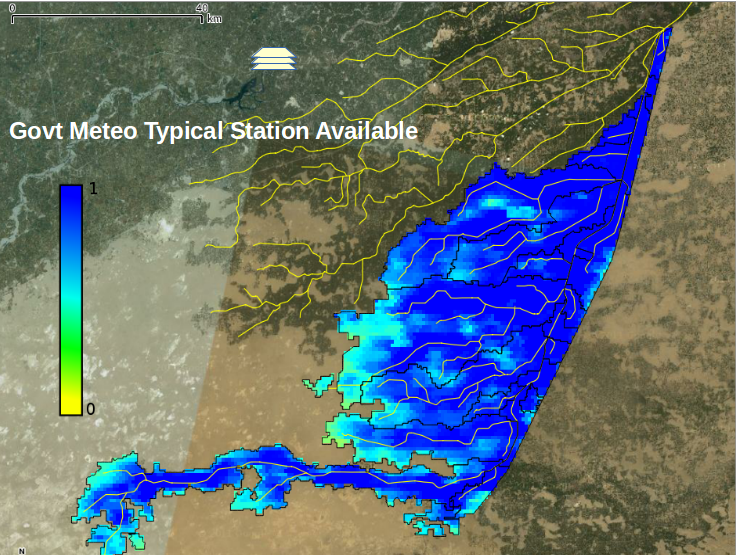
\includegraphics[width=10cm]{MWS_v1_deltaT_rationale_0}
%\end{center}
%
%\end{frame}
%
%%%%%%%%%%%%%%%%%%%%%%%%%%%%%%%%%%%%%%%%%%%%%%%%%%%%%%%%%%%%%%%%%%%%%
%\begin{frame}[fragile]{Rationale}
%
%\begin{center}
%  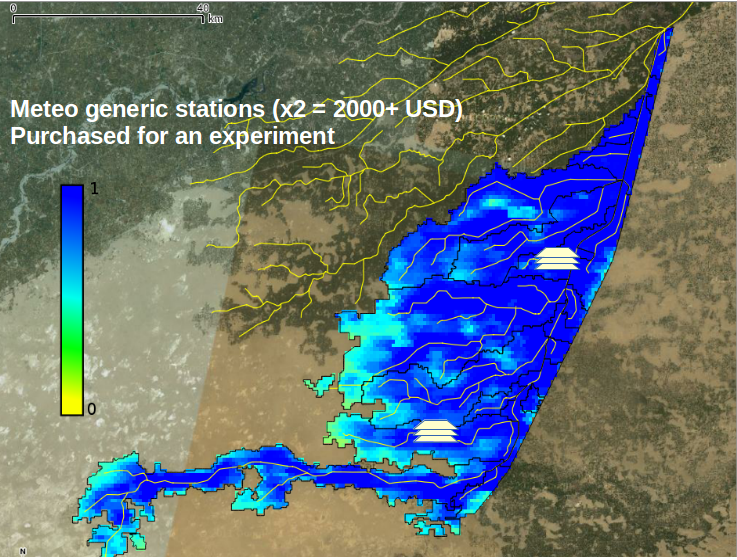
\includegraphics[width=10cm]{MWS_v1_deltaT_rationale_1}
%\end{center}
%
%\end{frame}
%
%%%%%%%%%%%%%%%%%%%%%%%%%%%%%%%%%%%%%%%%%%%%%%%%%%%%%%%%%%%%%%%%%%%%%
%\begin{frame}[fragile]{Rationale}
%
%\begin{center}
%  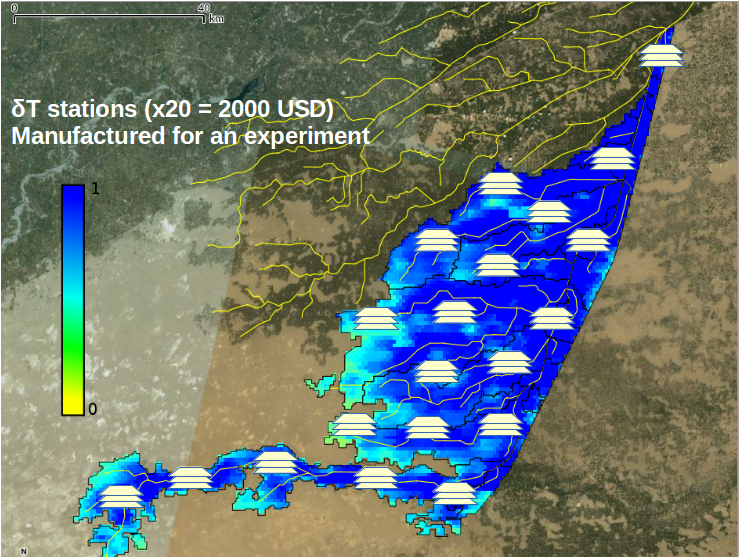
\includegraphics[width=10cm]{MWS_v1_deltaT_rationale_2}
%\end{center}
%
%\end{frame}
%
%\subsection{ $\delta T$ Tower}
%%%%%%%%%%%%%%%%%%%%%%%%%%%%%%%%%%%%%%%%%%%%%%%%%%%%%%%%%%%%%%%%%%%%%
%\begin{frame}[fragile]{Open Source Hardware Micro Weather Station v0}
%
%\textbf{Micro Weather Station v0:}\\
%Temperature Profiler for ET models calibration
%\vspace{5mm}
%\begin{itemize}
% \item Arduino Pro 3.3V
% \item Water-proof Digital Temperature Sensors
% \item Li-ion Battery + Solar Panel
% \item OpenLog data logger with SD card
% \item Cost $<$ 100 USD
%\end{itemize}
%\begin{flushright}
%  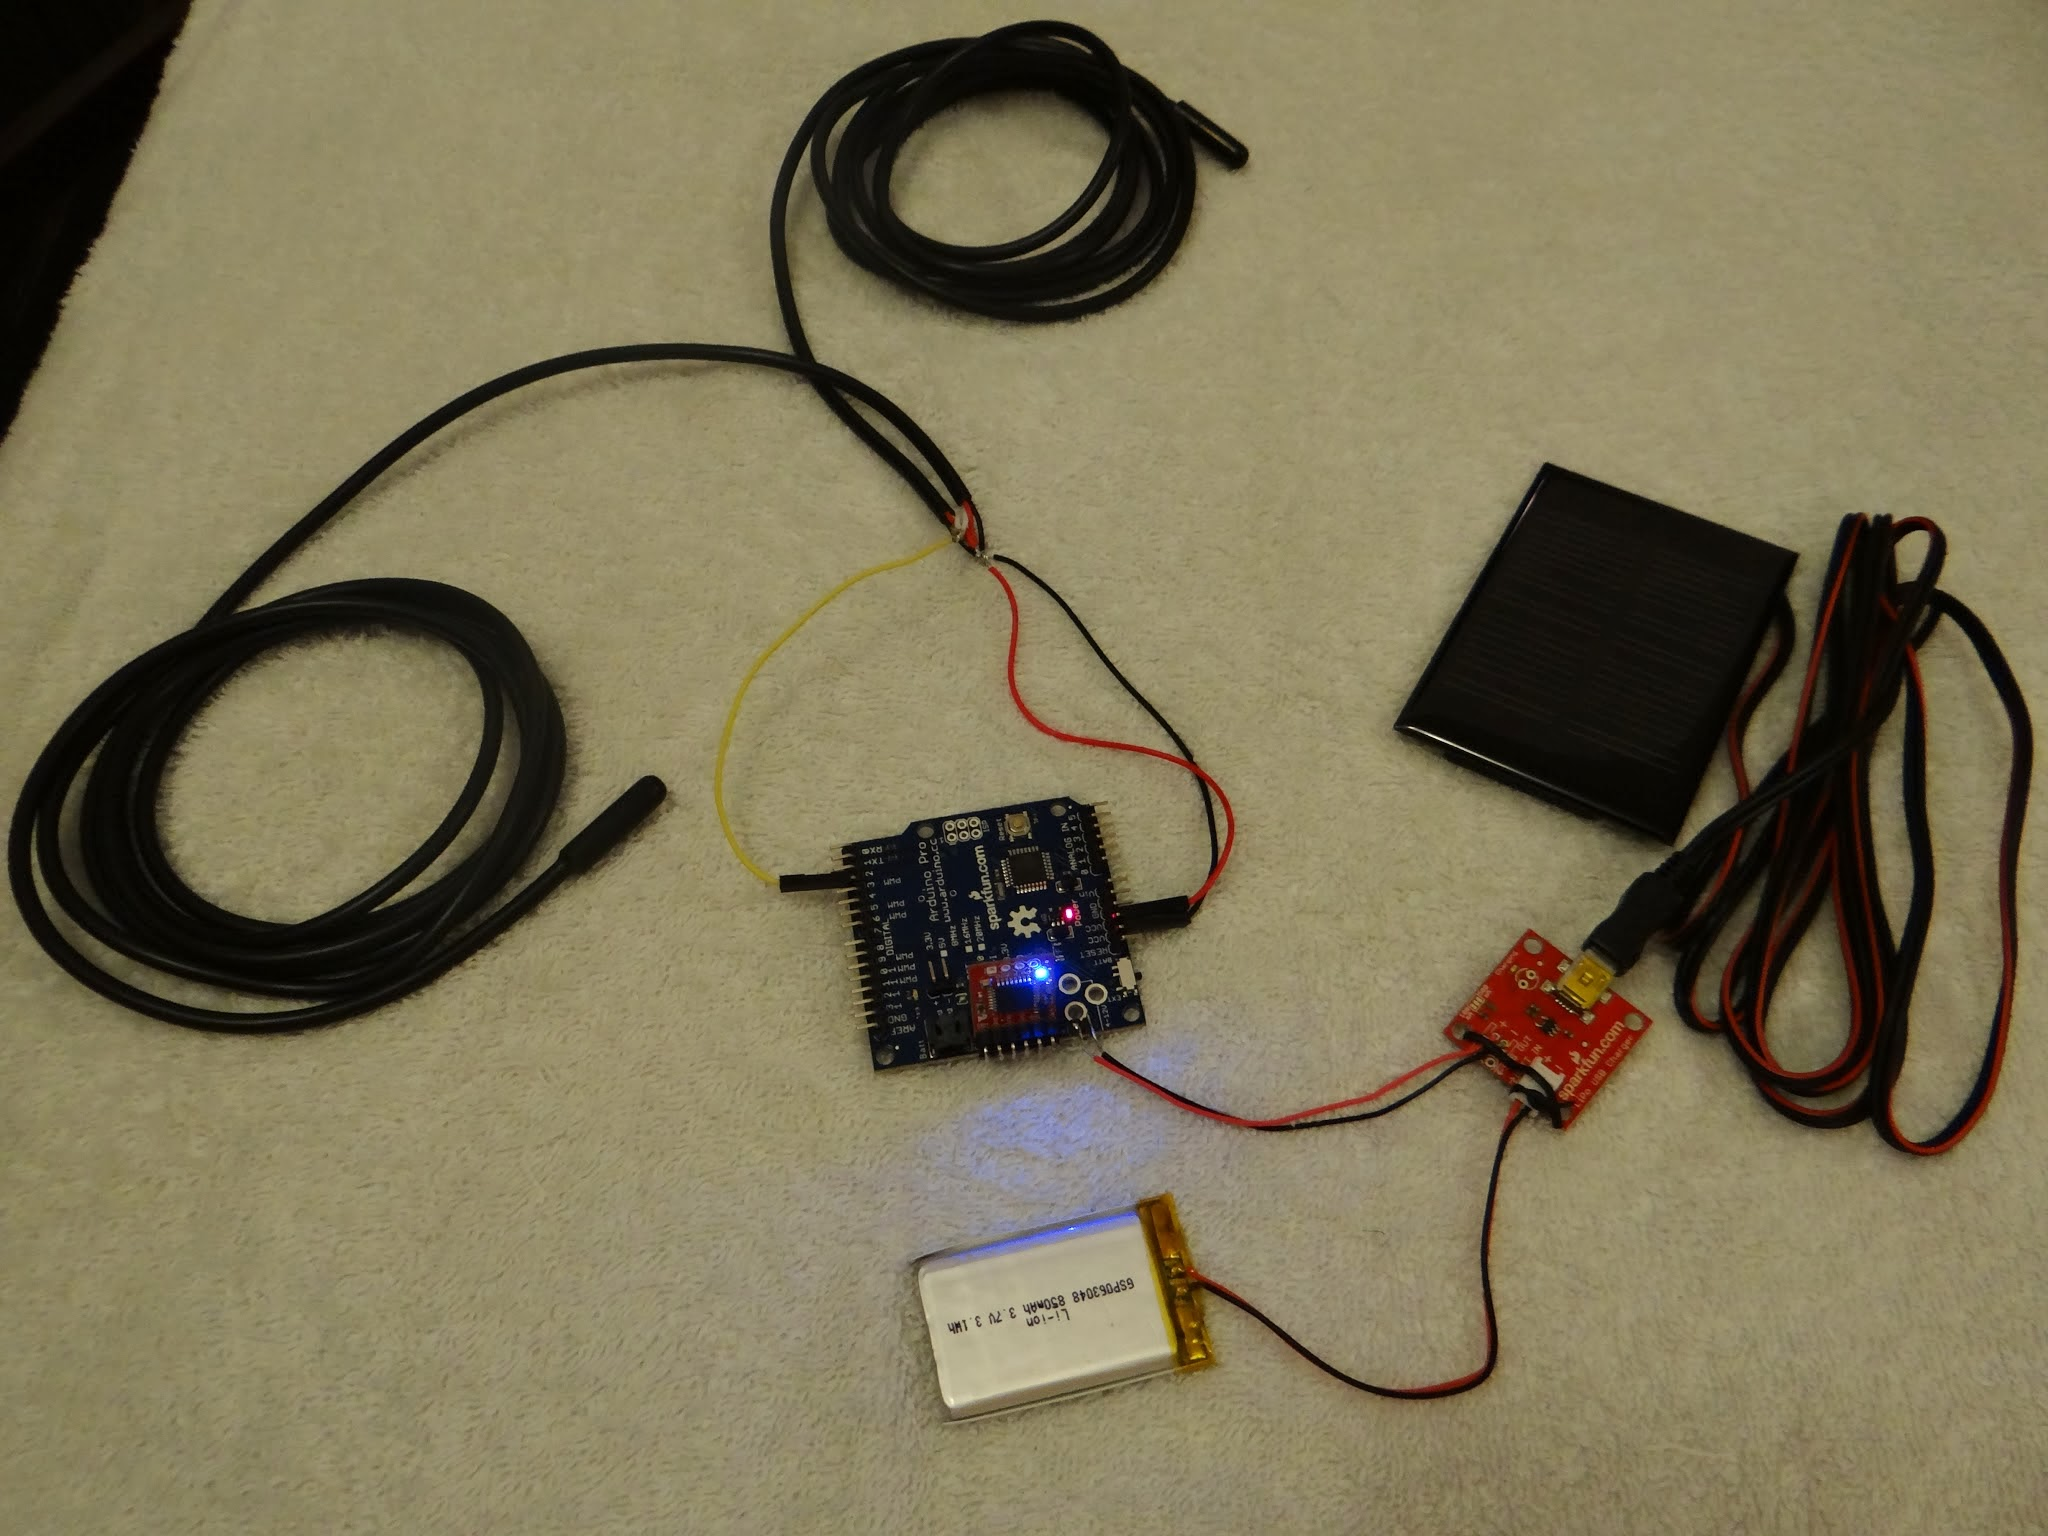
\includegraphics[width=5cm]{MWS}
%  \hspace{5mm}
%  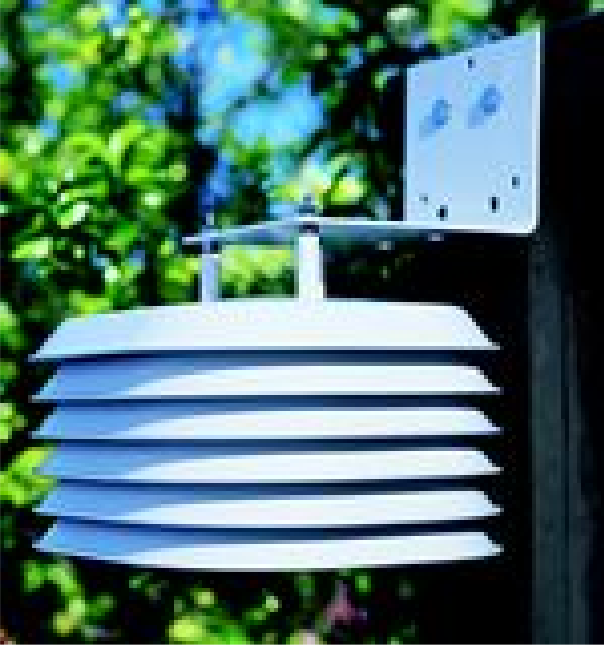
\includegraphics[width=2cm]{MWS_radshield}
%\end{flushright}
%\end{frame}
%
%\subsection{ $\delta T$ parts}
%%%%%%%%%%%%%%%%%%%%%%%%%%%%%%%%%%%%%%%%%%%%%%%%%%%%%%%%%%%%%%%%%%%%%
%\begin{frame}[fragile]{Open Source Hardware Micro Weather Station v0}
%
%\begin{center}
%OpenLog + Arduino Pro\\
%\vspace{5mm}
%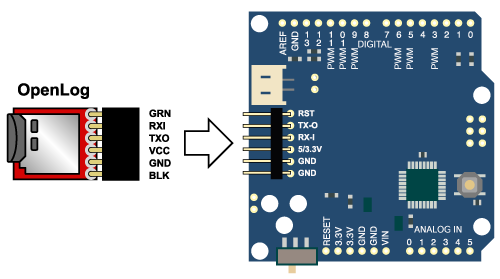
\includegraphics[width=5cm]{Arduino_OpenLog}
%\end{center}
%
%\begin{flushright}
%  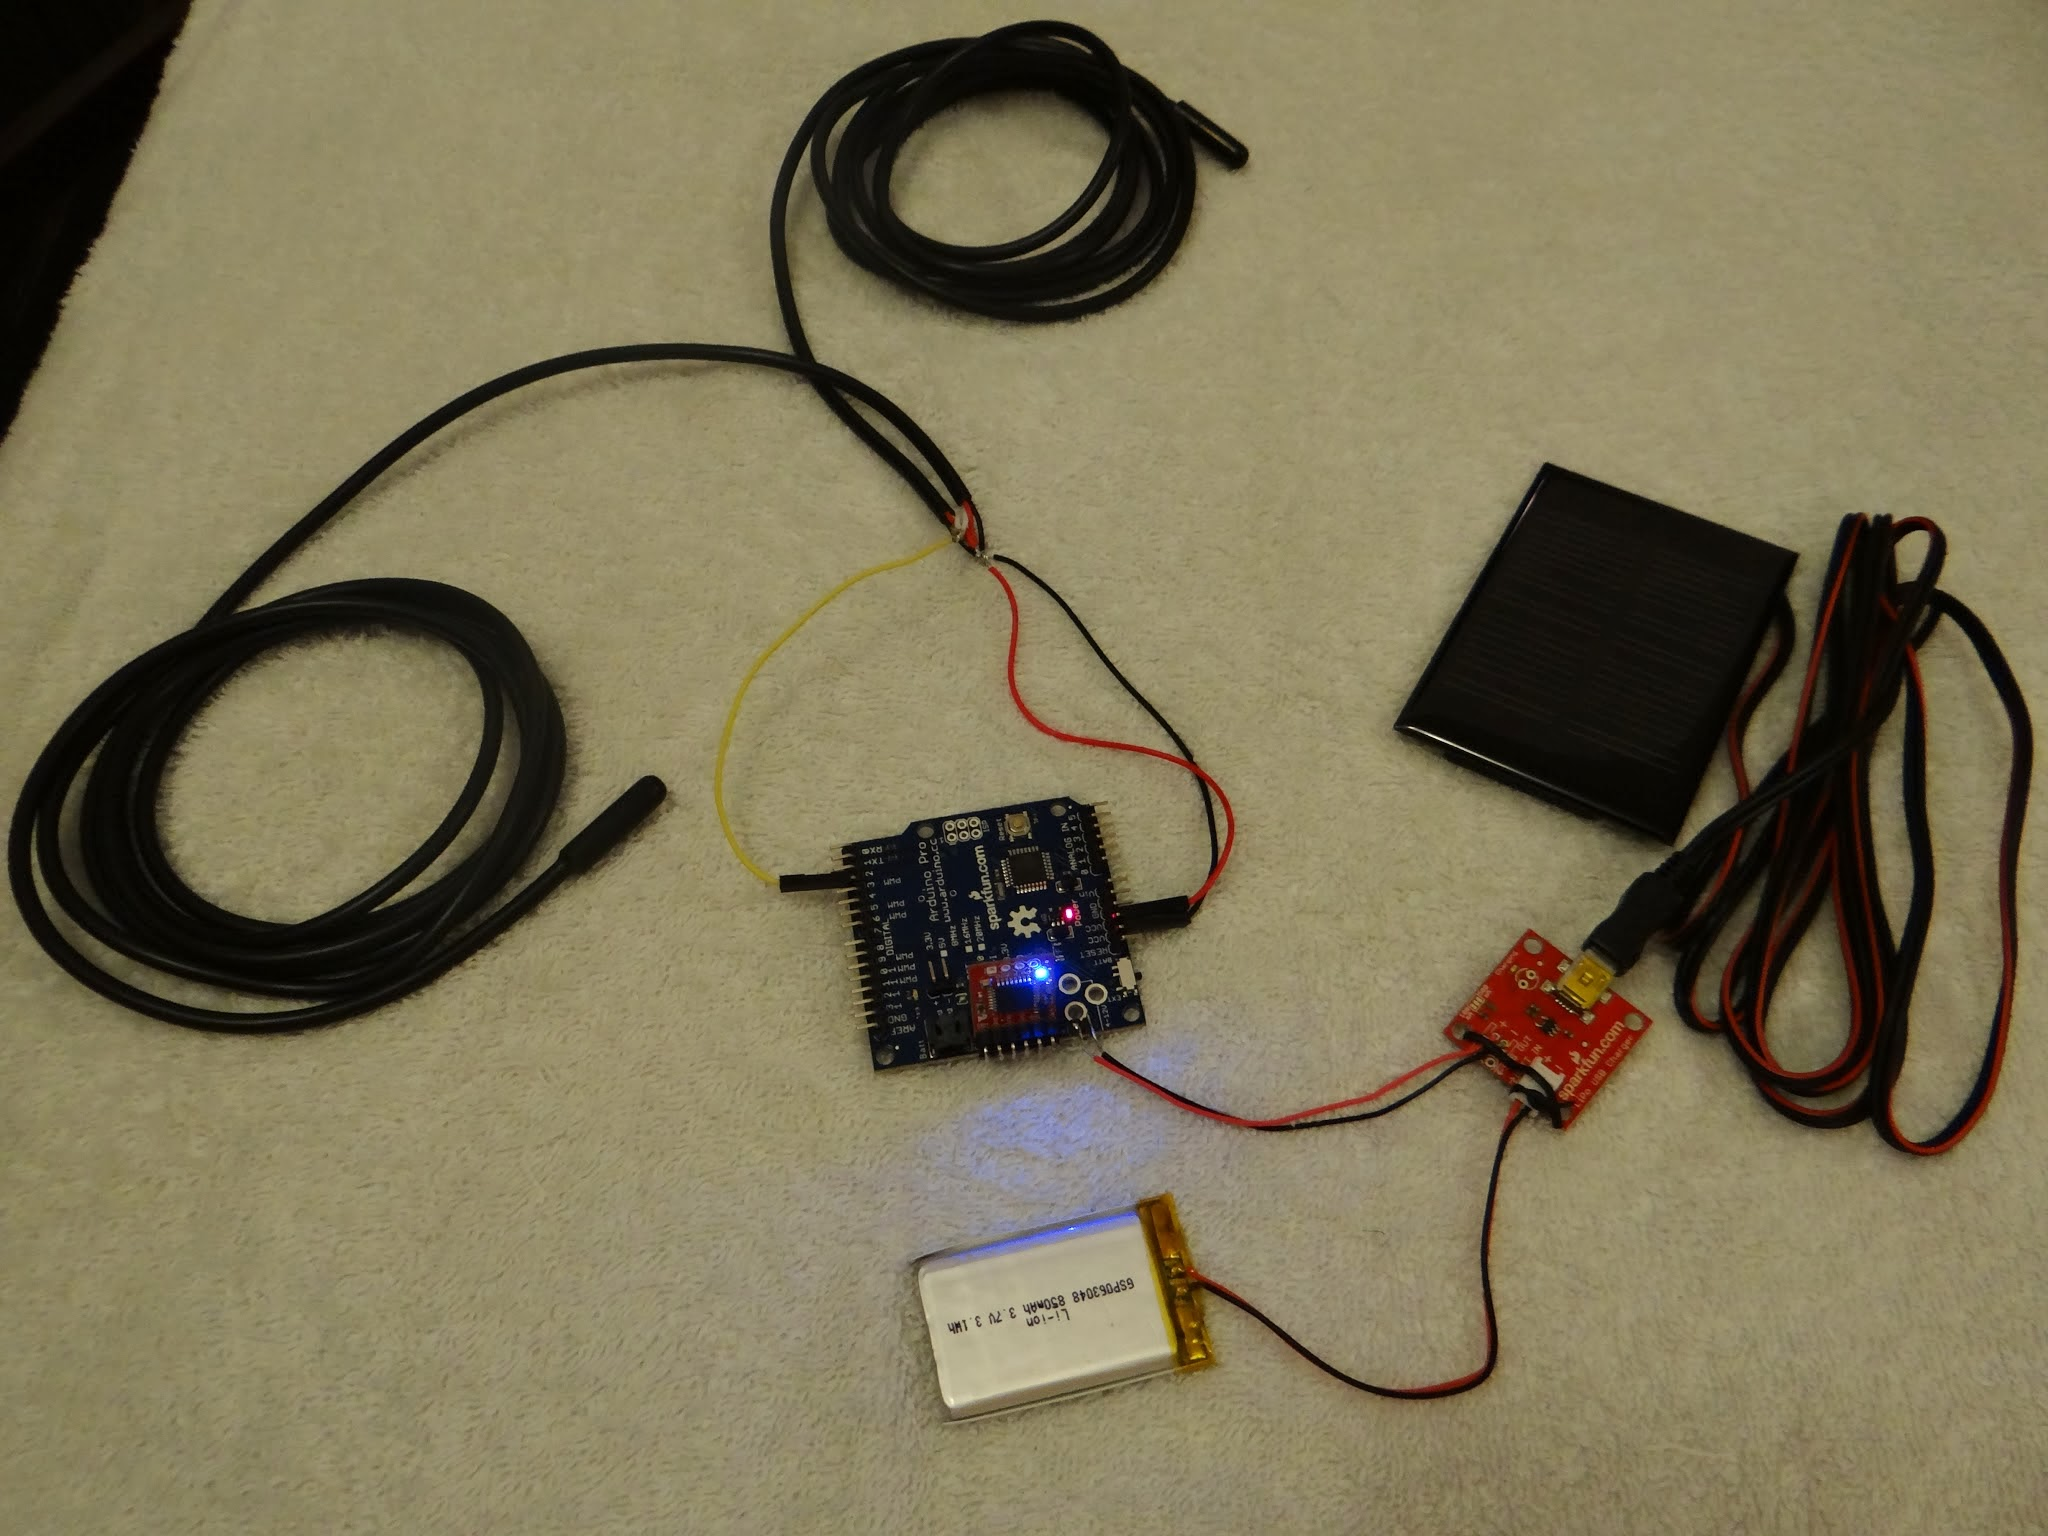
\includegraphics[width=5cm]{MWS}
%  \hspace{5mm}
%  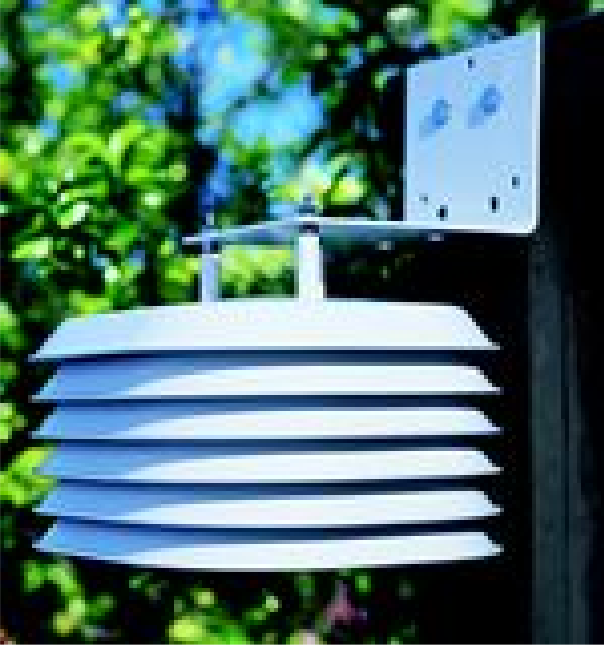
\includegraphics[width=2cm]{MWS_radshield}
%\end{flushright}
%\end{frame}
%
%\subsection{ $\delta T$ Setup}
%%%%%%%%%%%%%%%%%%%%%%%%%%%%%%%%%%%%%%%%%%%%%%%%%%%%%%%%%%%%%%%%%%%%%
%\begin{frame}[fragile]{MWS Setup}
%
%\begin{center}
% 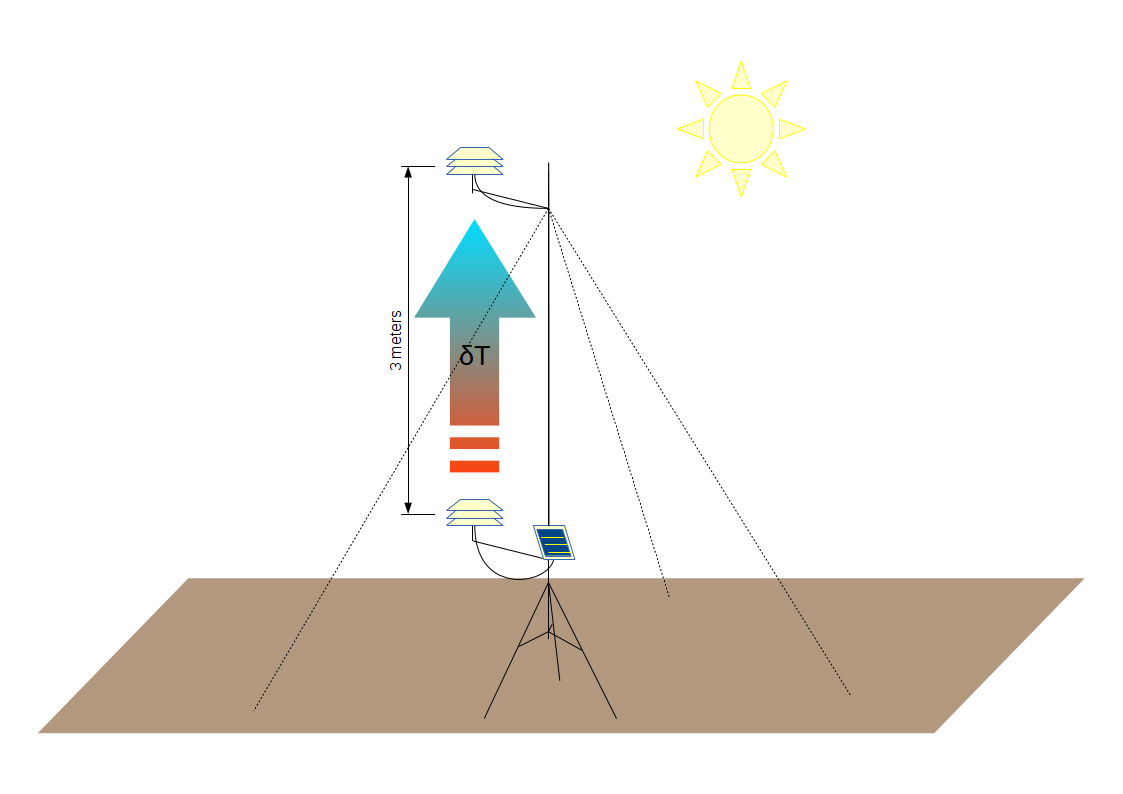
\includegraphics[width=10cm]{MWS_v1_deltaT_sketch_hot}
%\end{center}
%
%\end{frame}
%
%%%%%%%%%%%%%%%%%%%%%%%%%%%%%%%%%%%%%%%%%%%%%%%%%%%%%%%%%%%%%%%%%%%%%
%\begin{frame}[fragile]{ $\delta T$ Setup}
%
%\begin{center}
% 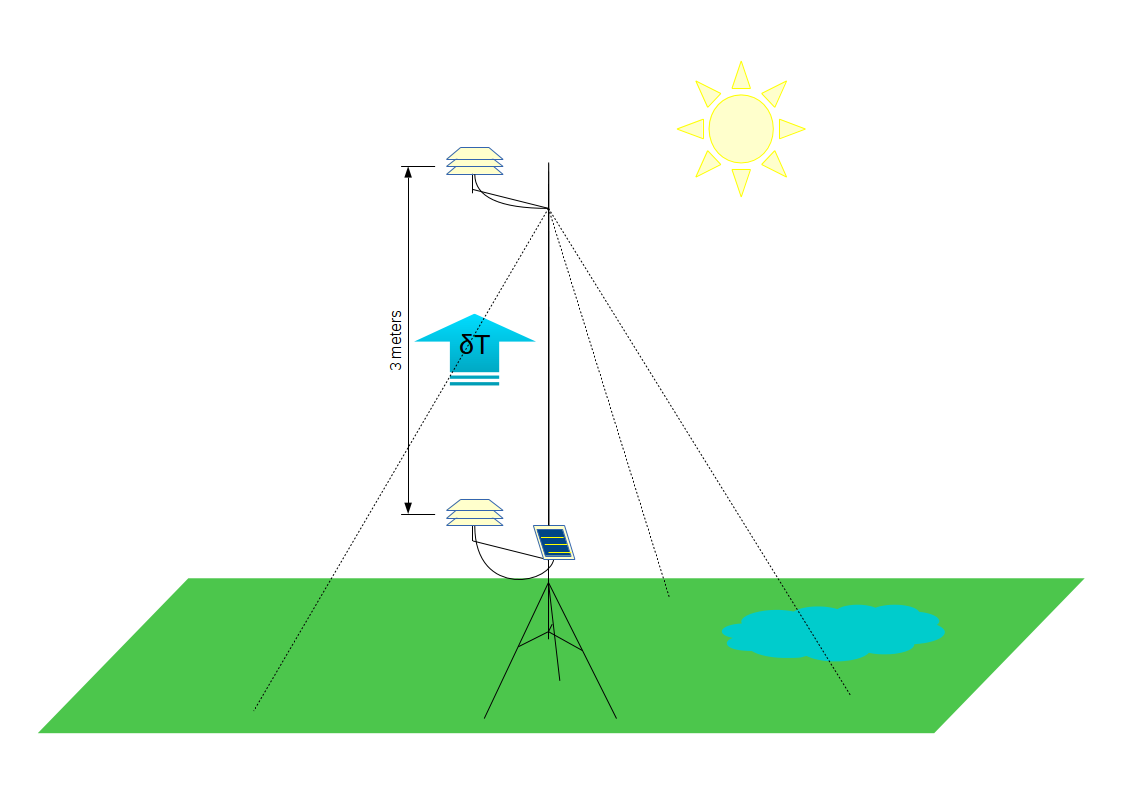
\includegraphics[width=10cm]{MWS_v1_deltaT_sketch_cold}
%\end{center}
%
%\end{frame}

\section{ MWS Tower}
%%%%%%%%%%%%%%%%%%%%%%%%%%%%%%%%%%%%%%%%%%%%%%%%%%%%%%%%%%%%%%%%%%%%
\begin{frame}[fragile]{Open Source Hardware Micro Weather Station v1}

\textbf{Micro Weather Station v1:}\\
Meteorological support for Irrigation Department in Sri Lanka, for faster management of rural reservoirs spilling in case of high rain intensity.
\vspace{5mm}
\begin{itemize}
 \item Lakduino (\href{www.lakduino.com}{\textit{www.lakduino.com}})
 \item Weather Sensor Board
 \item GPRS Modem Board
 \item Data logger with 16Gb micro-SD card
 \item Moto battery + Solar Panel
\end{itemize}
\begin{flushright}
  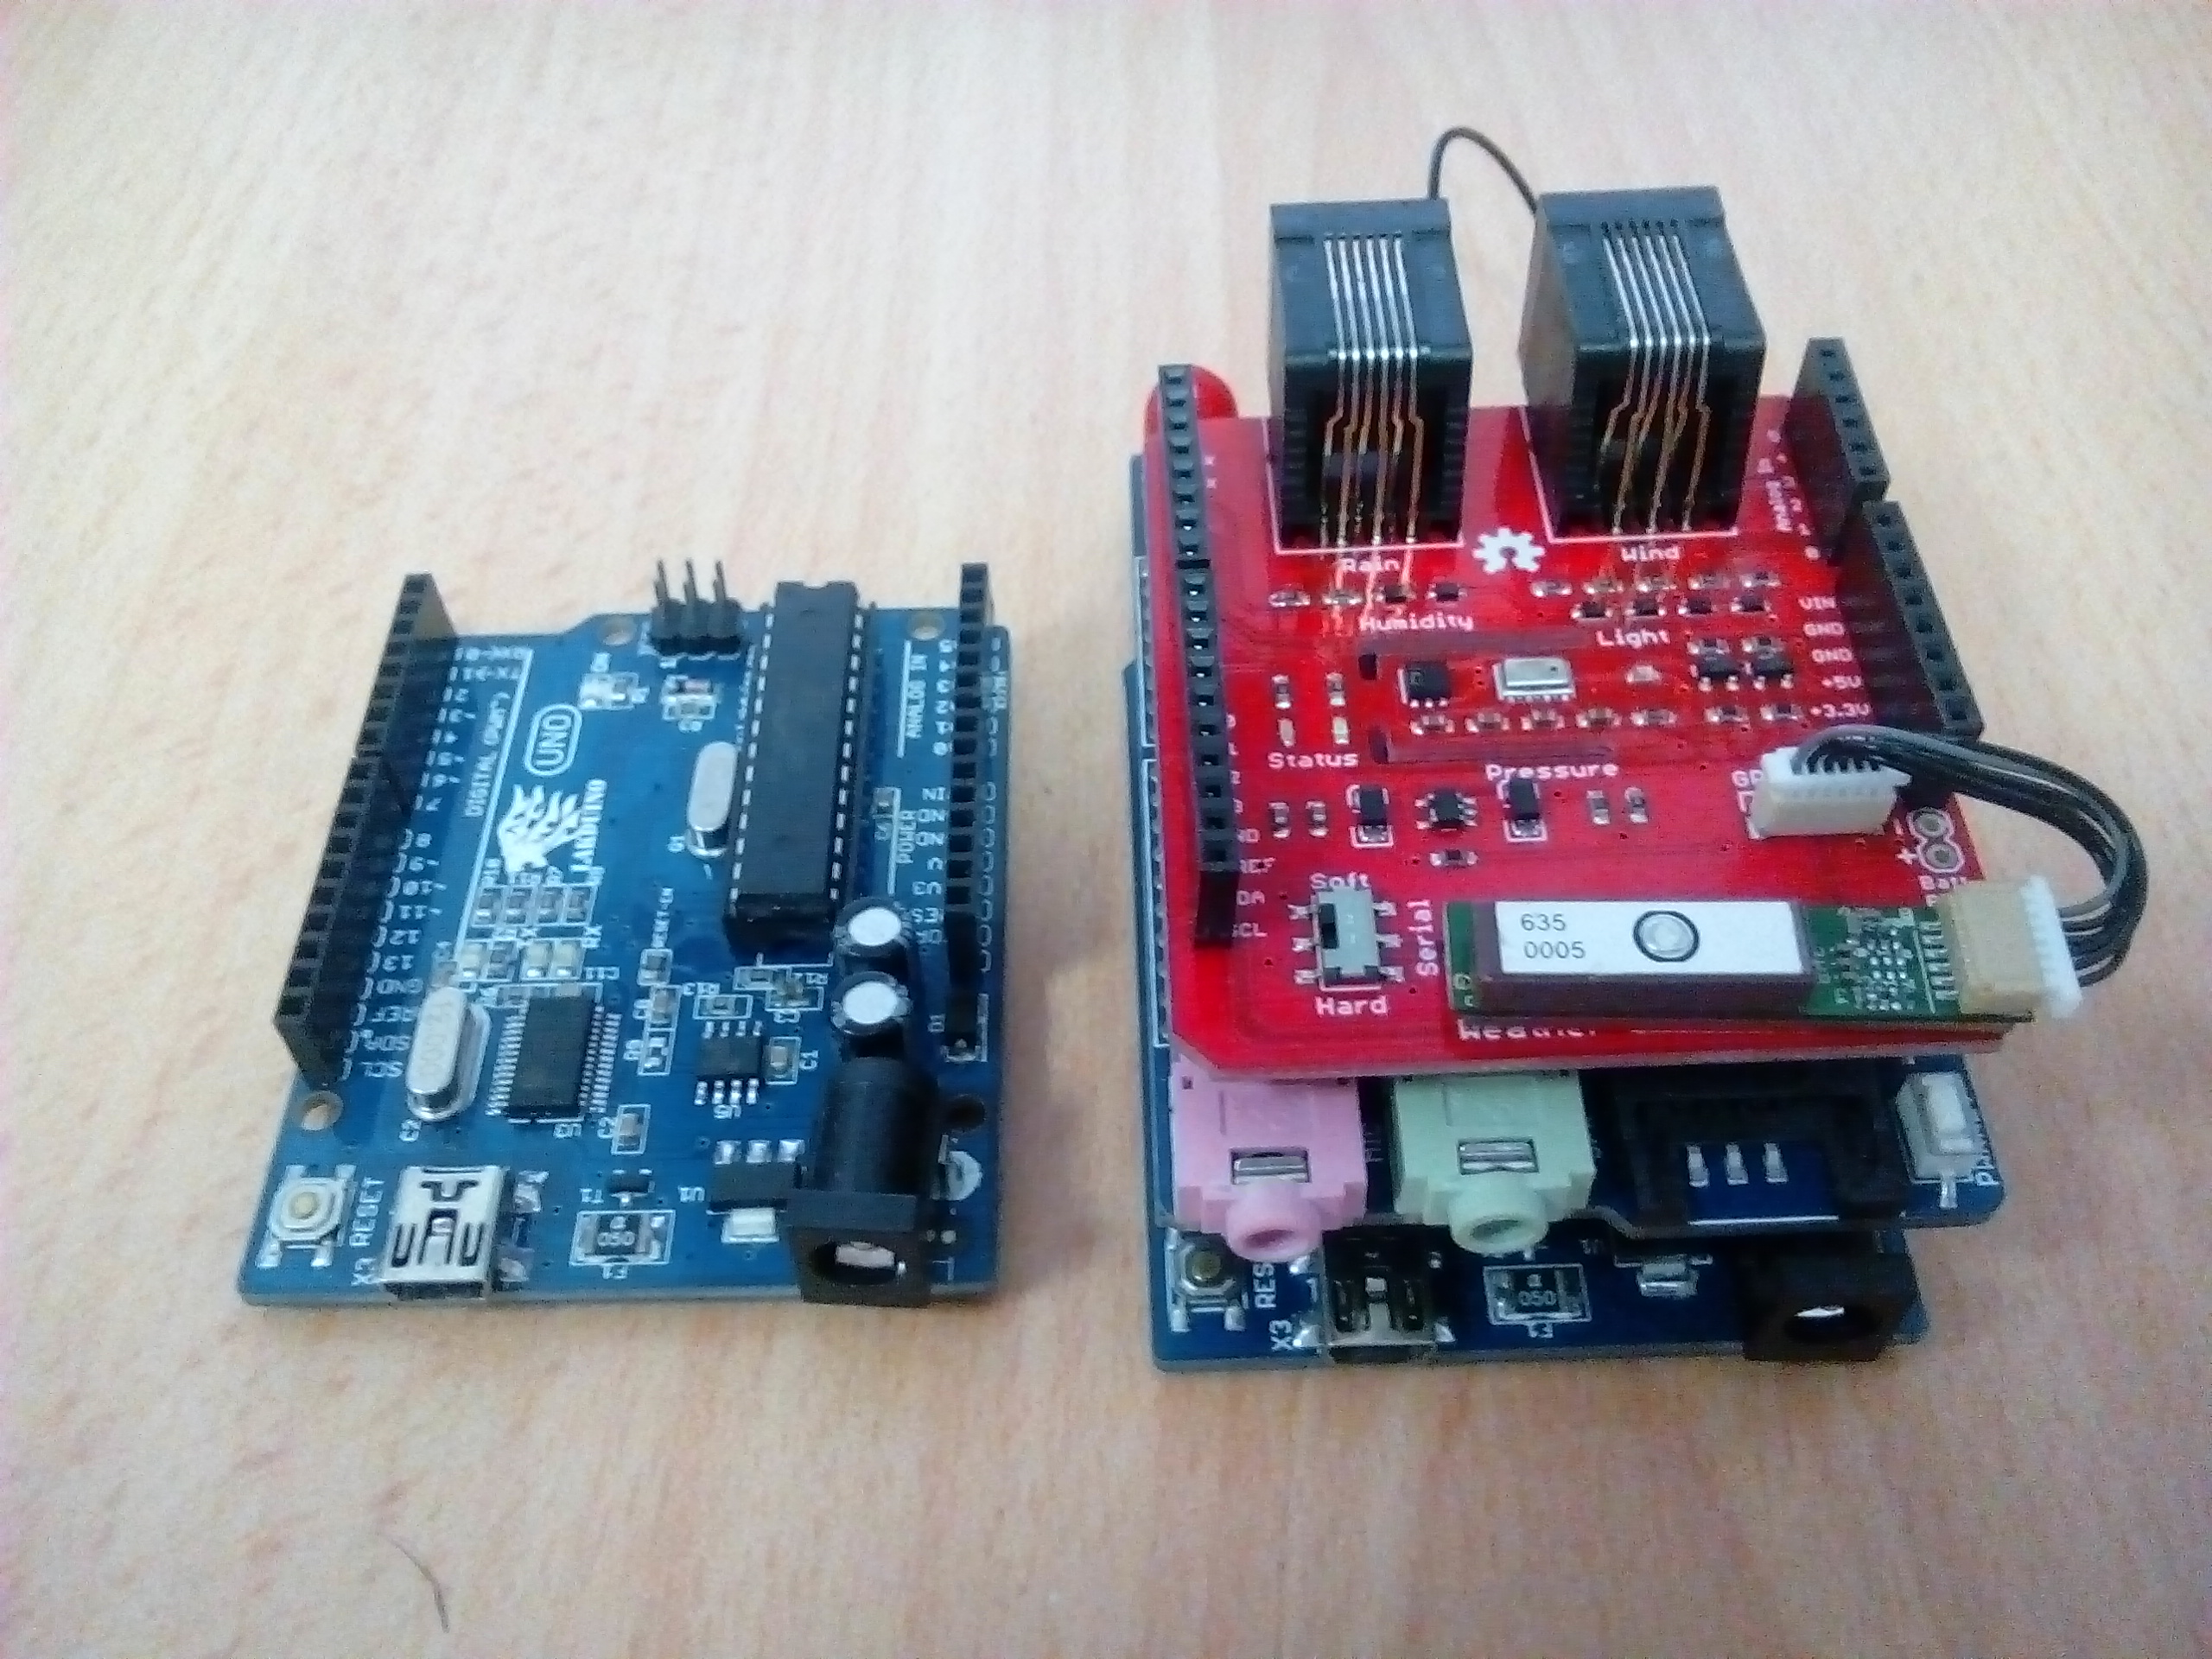
\includegraphics[width=5cm]{MWSv1}
  \hspace{5mm}
  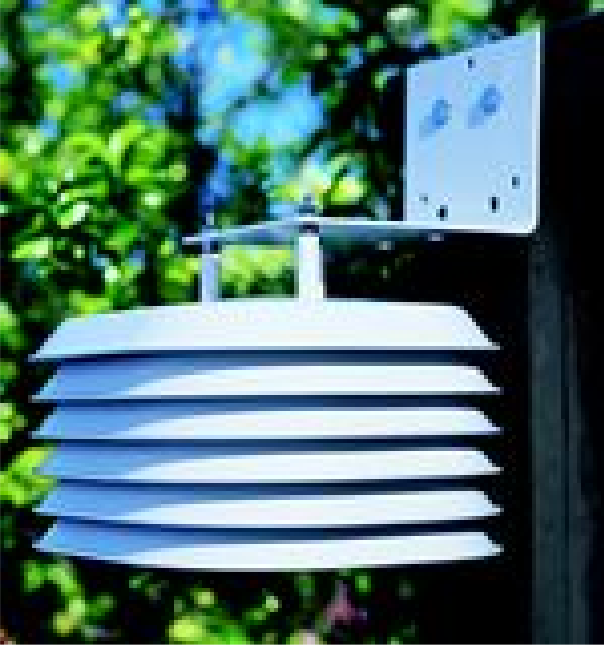
\includegraphics[width=2cm]{MWS_radshield}
\end{flushright}
\end{frame}

\subsection{Power Supply}
%%%%%%%%%%%%%%%%%%%%%%%%%%%%%%%%%%%%%%%%%%%%%%%%%%%%%%%%%%%%%%%%%%%%
\begin{frame}[fragile]{Open Source Hardware Micro Weather Station v0}

\begin{center}
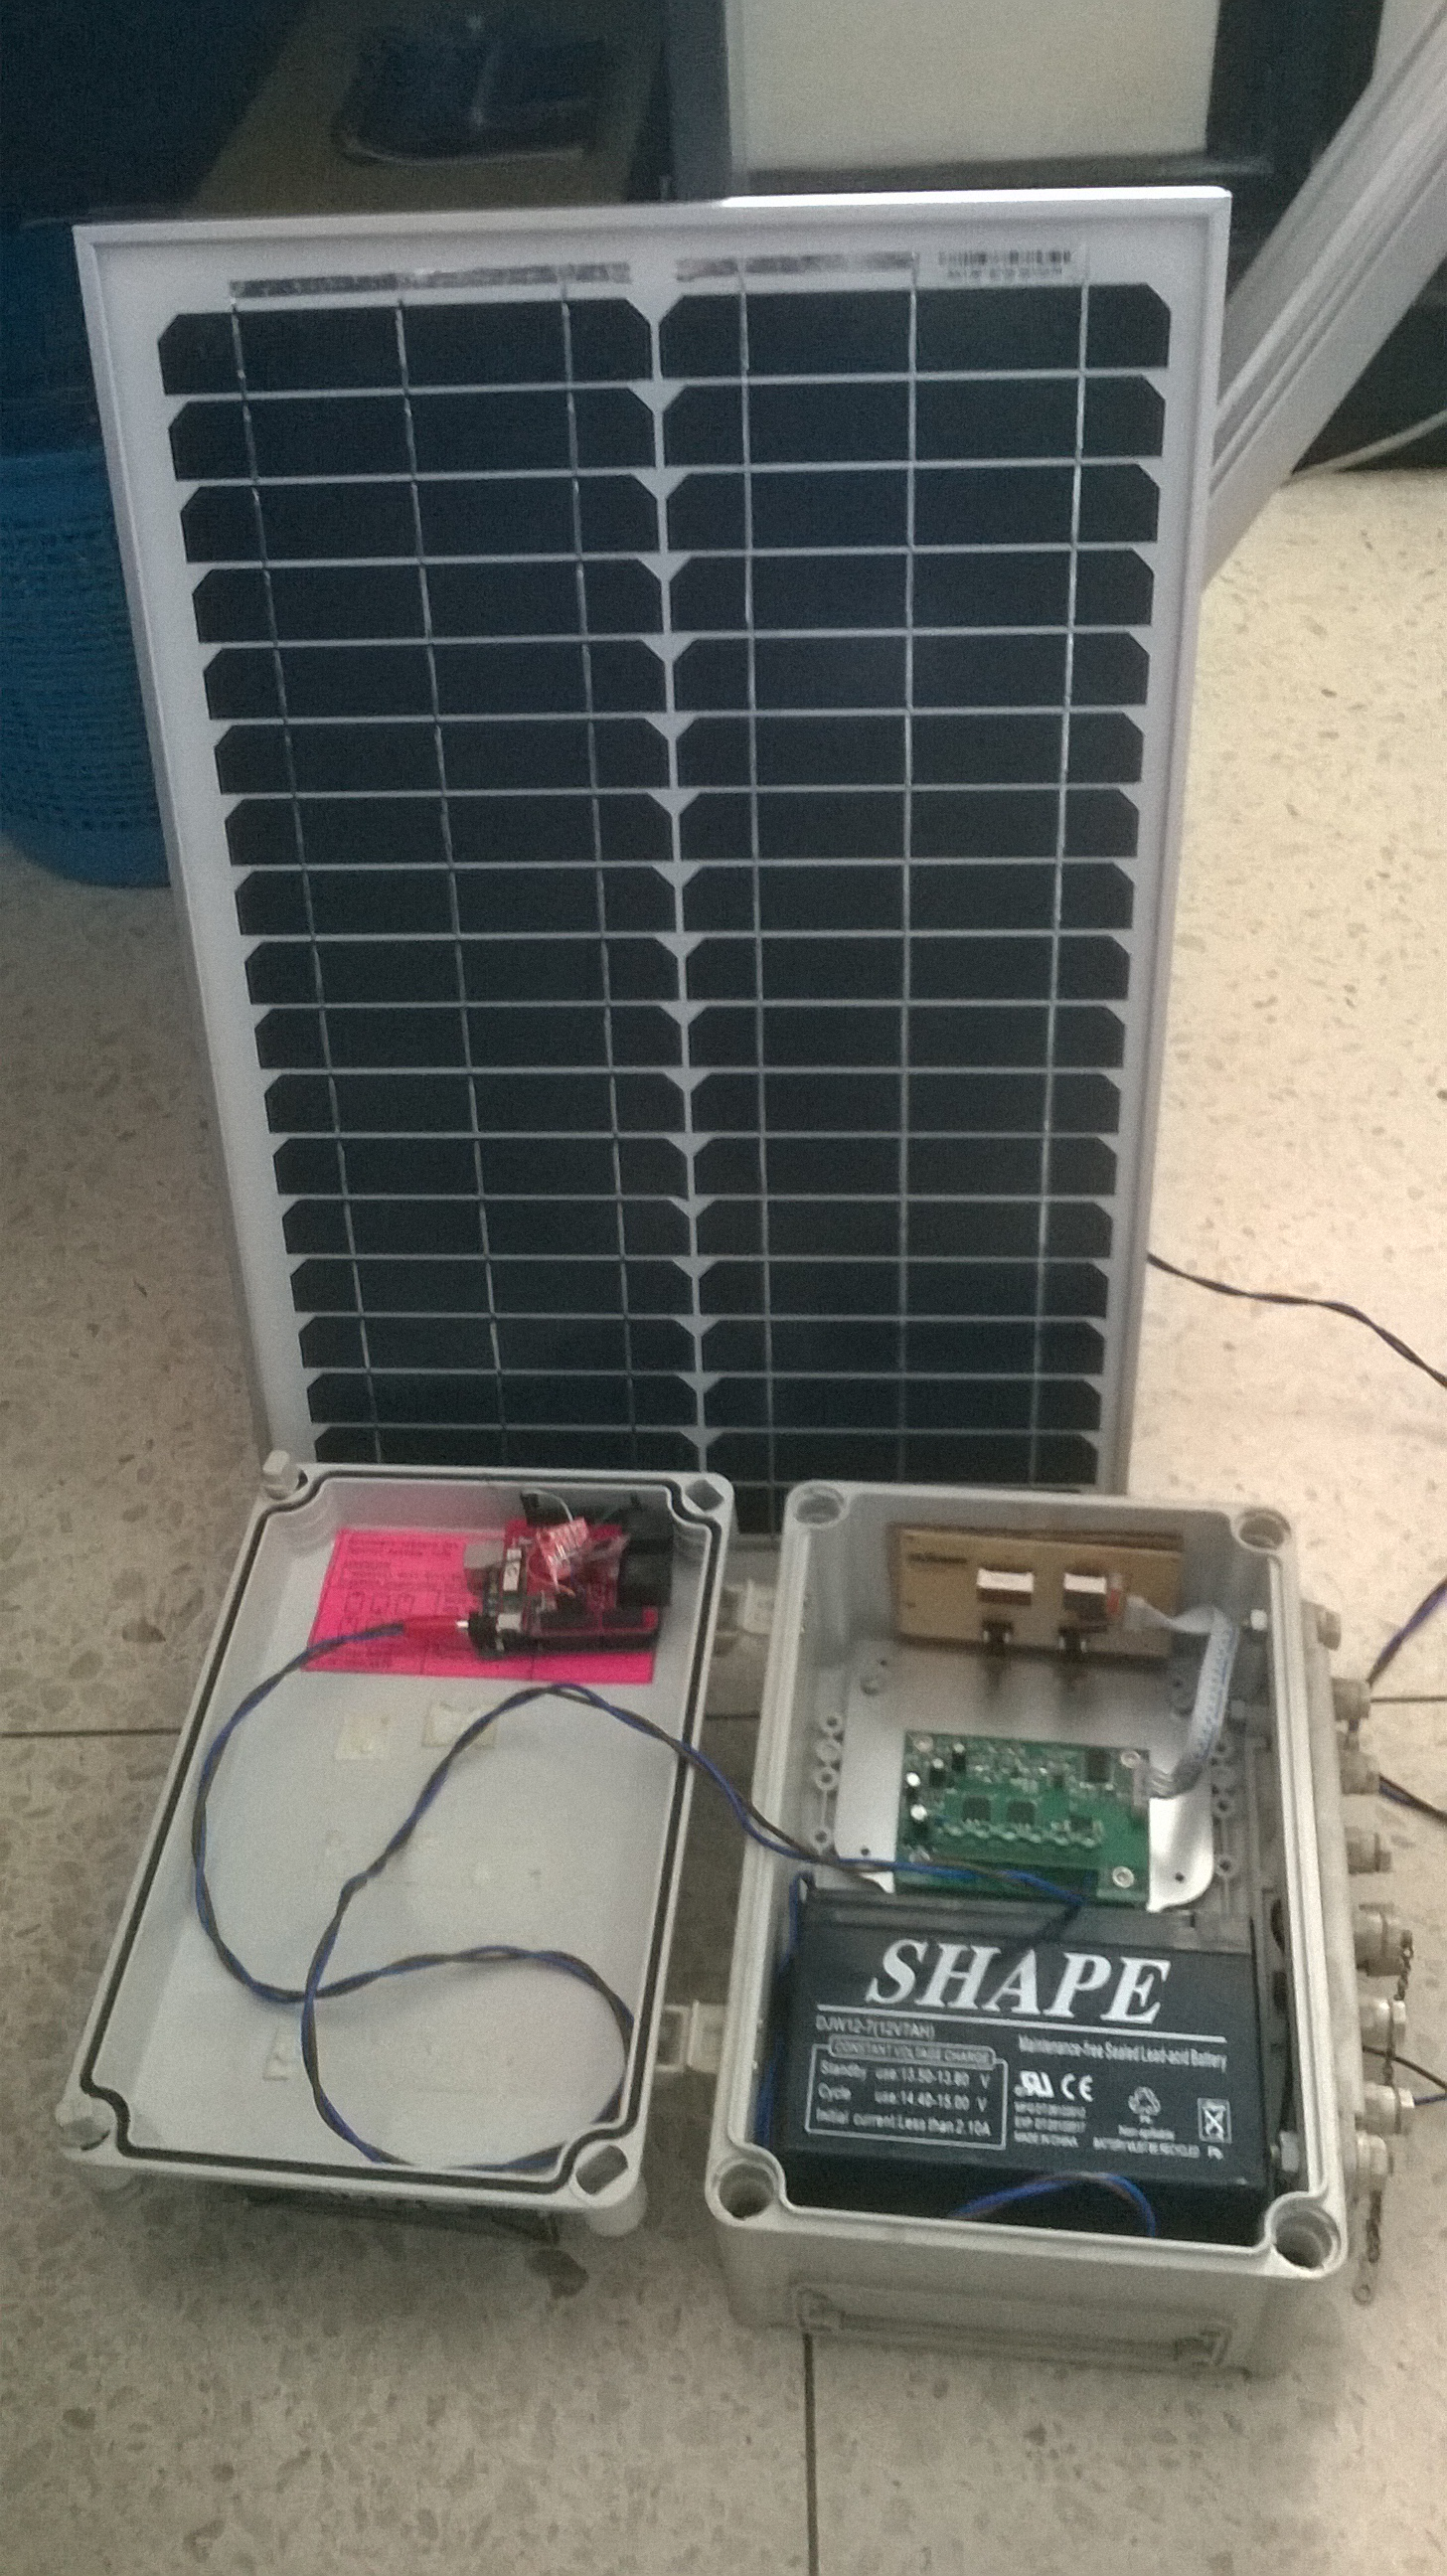
\includegraphics[width=4.5cm]{MWSv1_power}
\end{center}
\end{frame}

\subsection{Wind Sensors}
%%%%%%%%%%%%%%%%%%%%%%%%%%%%%%%%%%%%%%%%%%%%%%%%%%%%%%%%%%%%%%%%%%%%
\begin{frame}[fragile]{Wind Sensors}

\begin{center}
 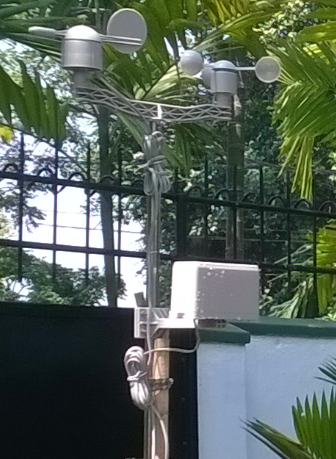
\includegraphics[width=7cm]{MWSv1_sensors}
\end{center}

\end{frame}

\subsection{Raingauge 1}
%%%%%%%%%%%%%%%%%%%%%%%%%%%%%%%%%%%%%%%%%%%%%%%%%%%%%%%%%%%%%%%%%%%%
\begin{frame}[fragile]{Raingauge 1}

\begin{center}
 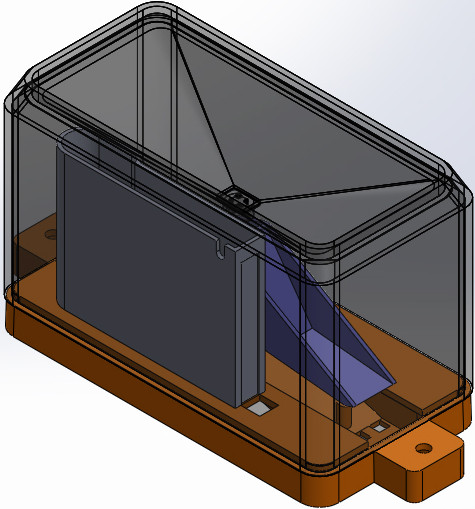
\includegraphics[width=6cm]{MWSv1_rain1}\\
\vspace{5mm}
Chinese made raingauge 3D view\\
from scion.lk
\end{center}

\end{frame}

\subsection{Raingauge 2}
%%%%%%%%%%%%%%%%%%%%%%%%%%%%%%%%%%%%%%%%%%%%%%%%%%%%%%%%%%%%%%%%%%%%
\begin{frame}[fragile]{Raingauge 2}

\begin{center}
 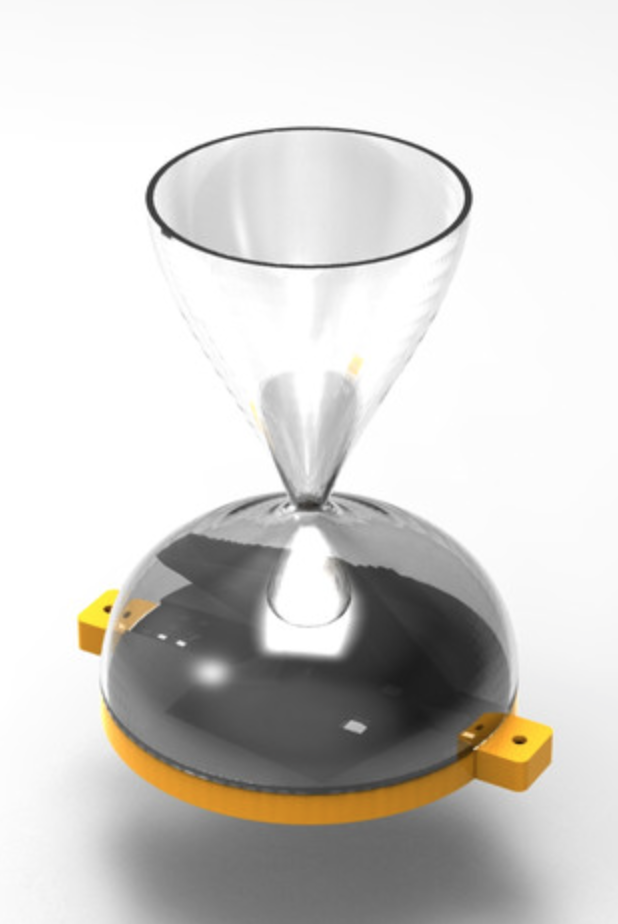
\includegraphics[width=4cm]{oshw_raingauge}\\
\vspace{5mm}
Public Domain, locally-designed rain gauge\\
https://grabcad.com/library/rain-gauge-design-1\\
from scion.lk
\end{center}
\end{frame}

\subsection{Electronics}
%%%%%%%%%%%%%%%%%%%%%%%%%%%%%%%%%%%%%%%%%%%%%%%%%%%%%%%%%%%%%%%%%%%%
\begin{frame}[fragile]{Electronics}

\begin{center}
 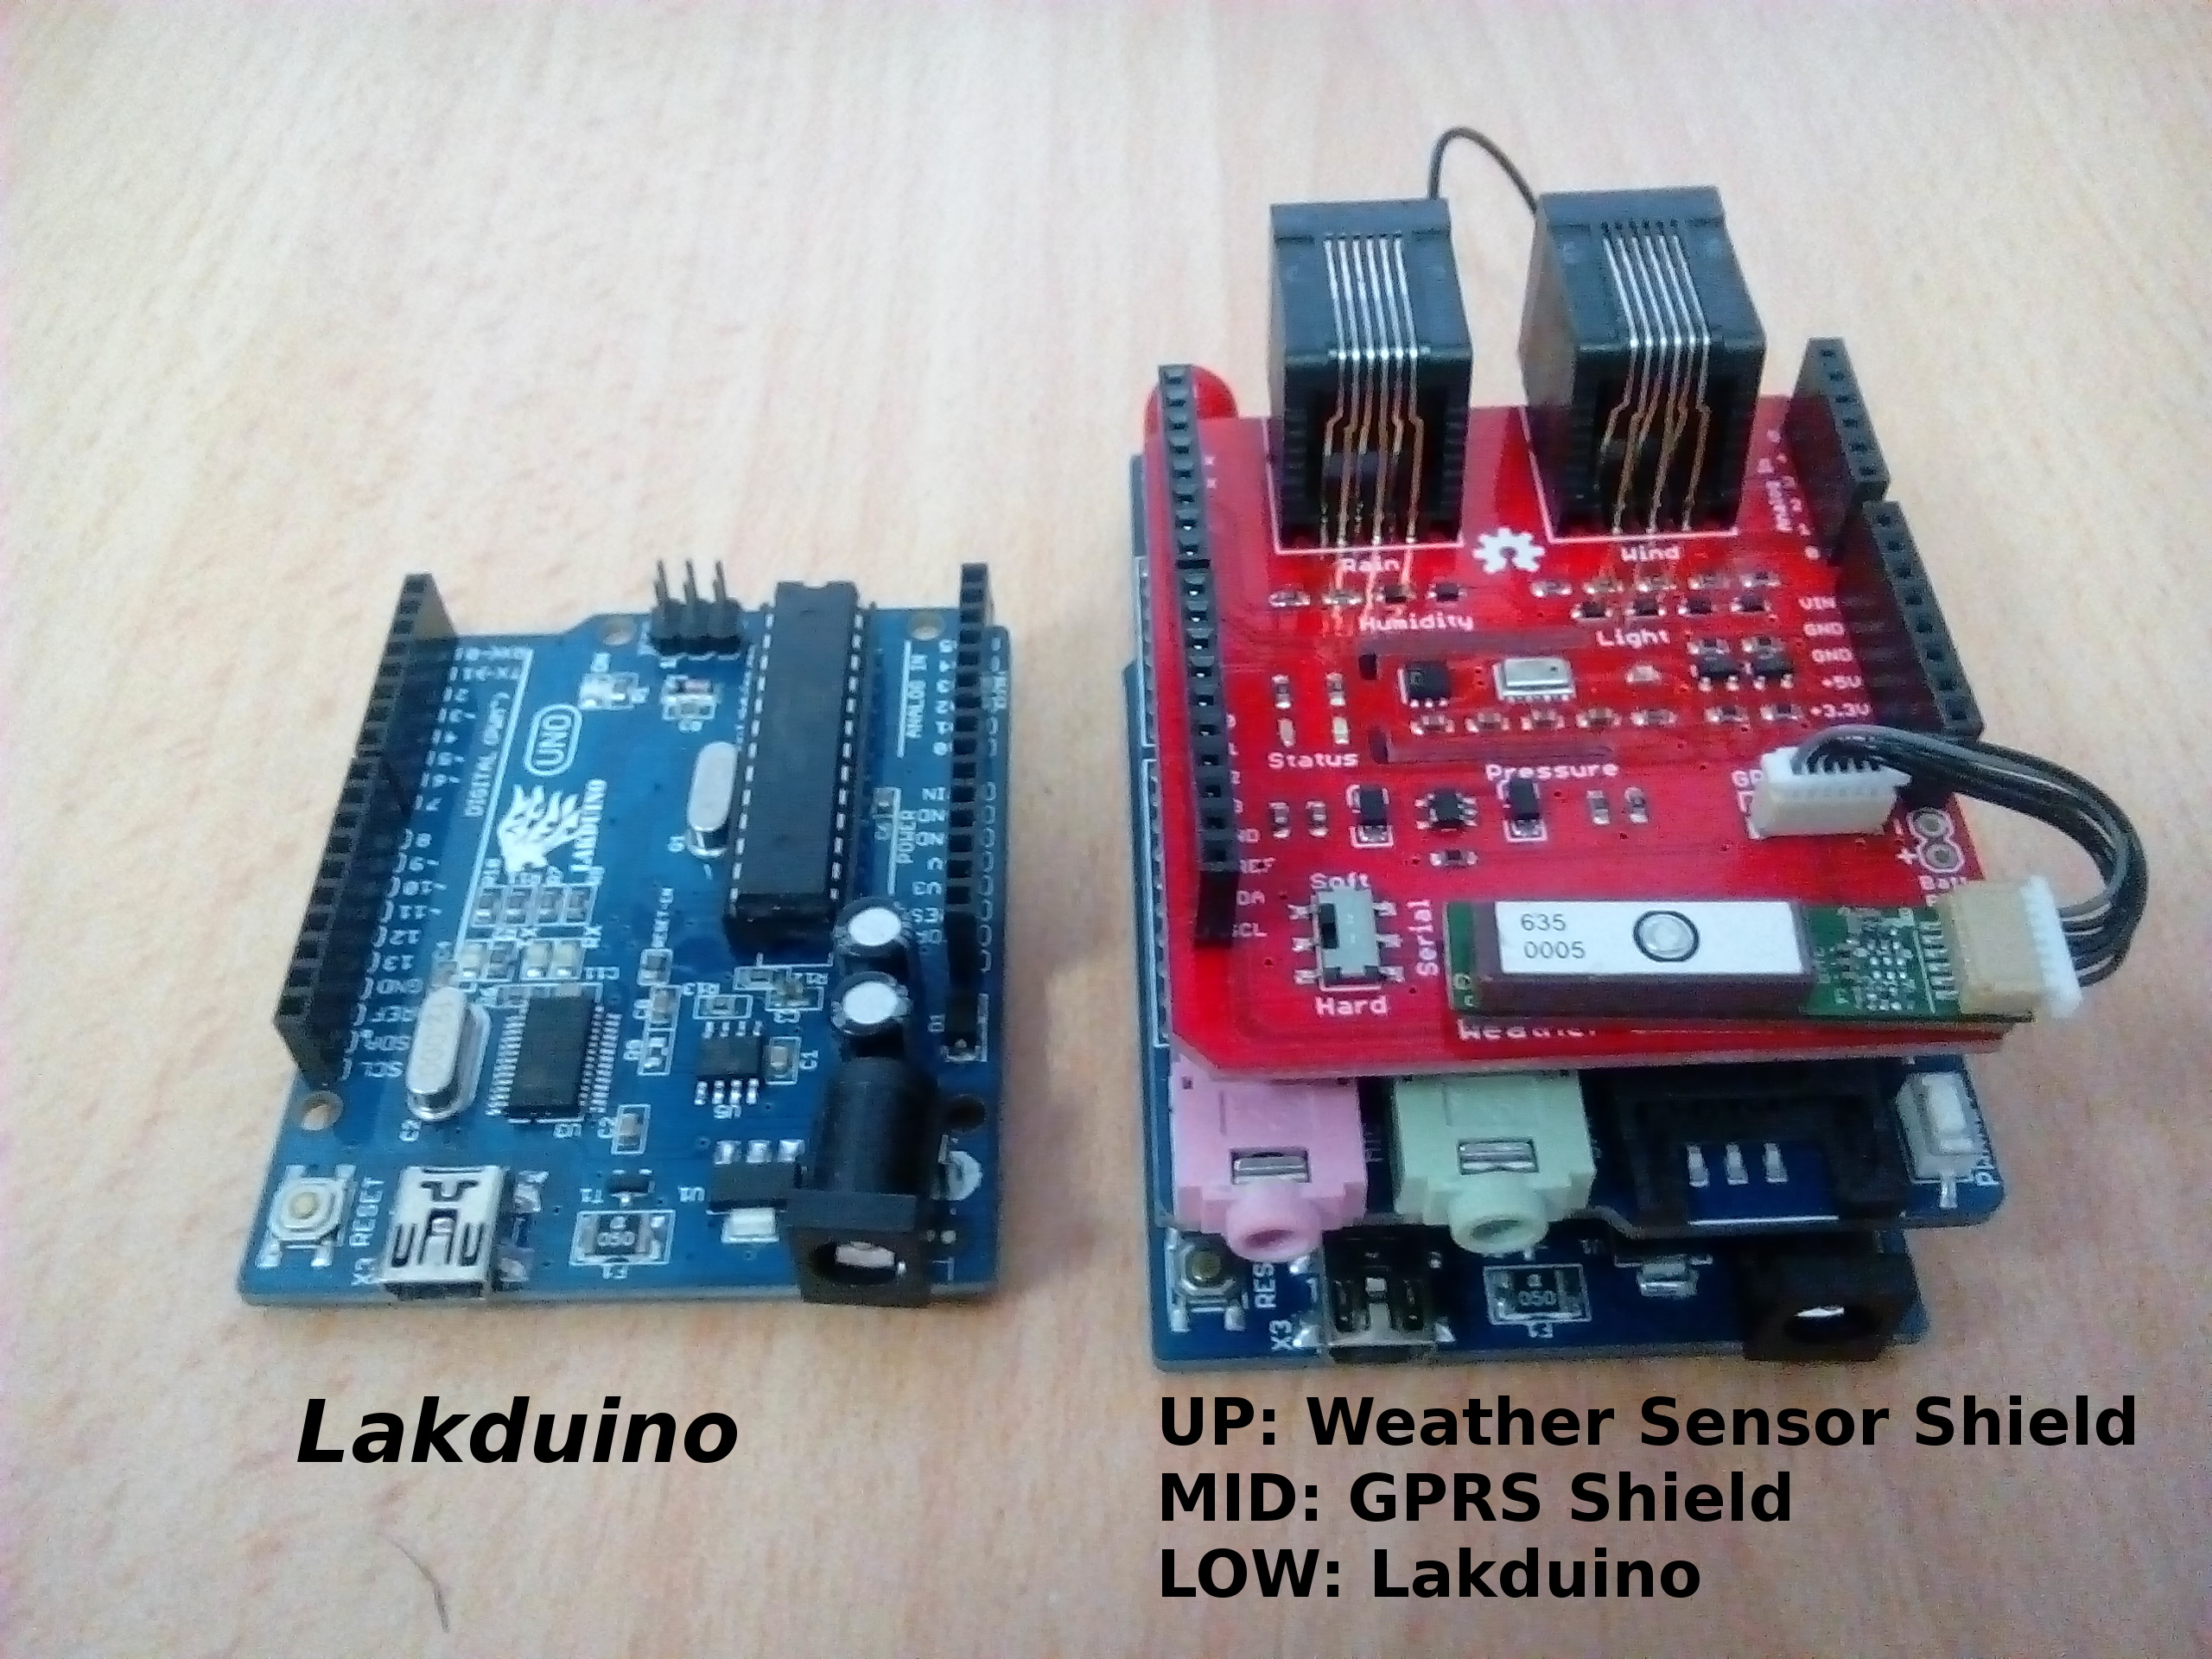
\includegraphics[width=10cm]{MWSv1_annotated}
\end{center}

\end{frame}

\subsection{Weather Shield}
%%%%%%%%%%%%%%%%%%%%%%%%%%%%%%%%%%%%%%%%%%%%%%%%%%%%%%%%%%%%%%%%%%%%
\begin{frame}[fragile]{Weather Shield}

\begin{center}
 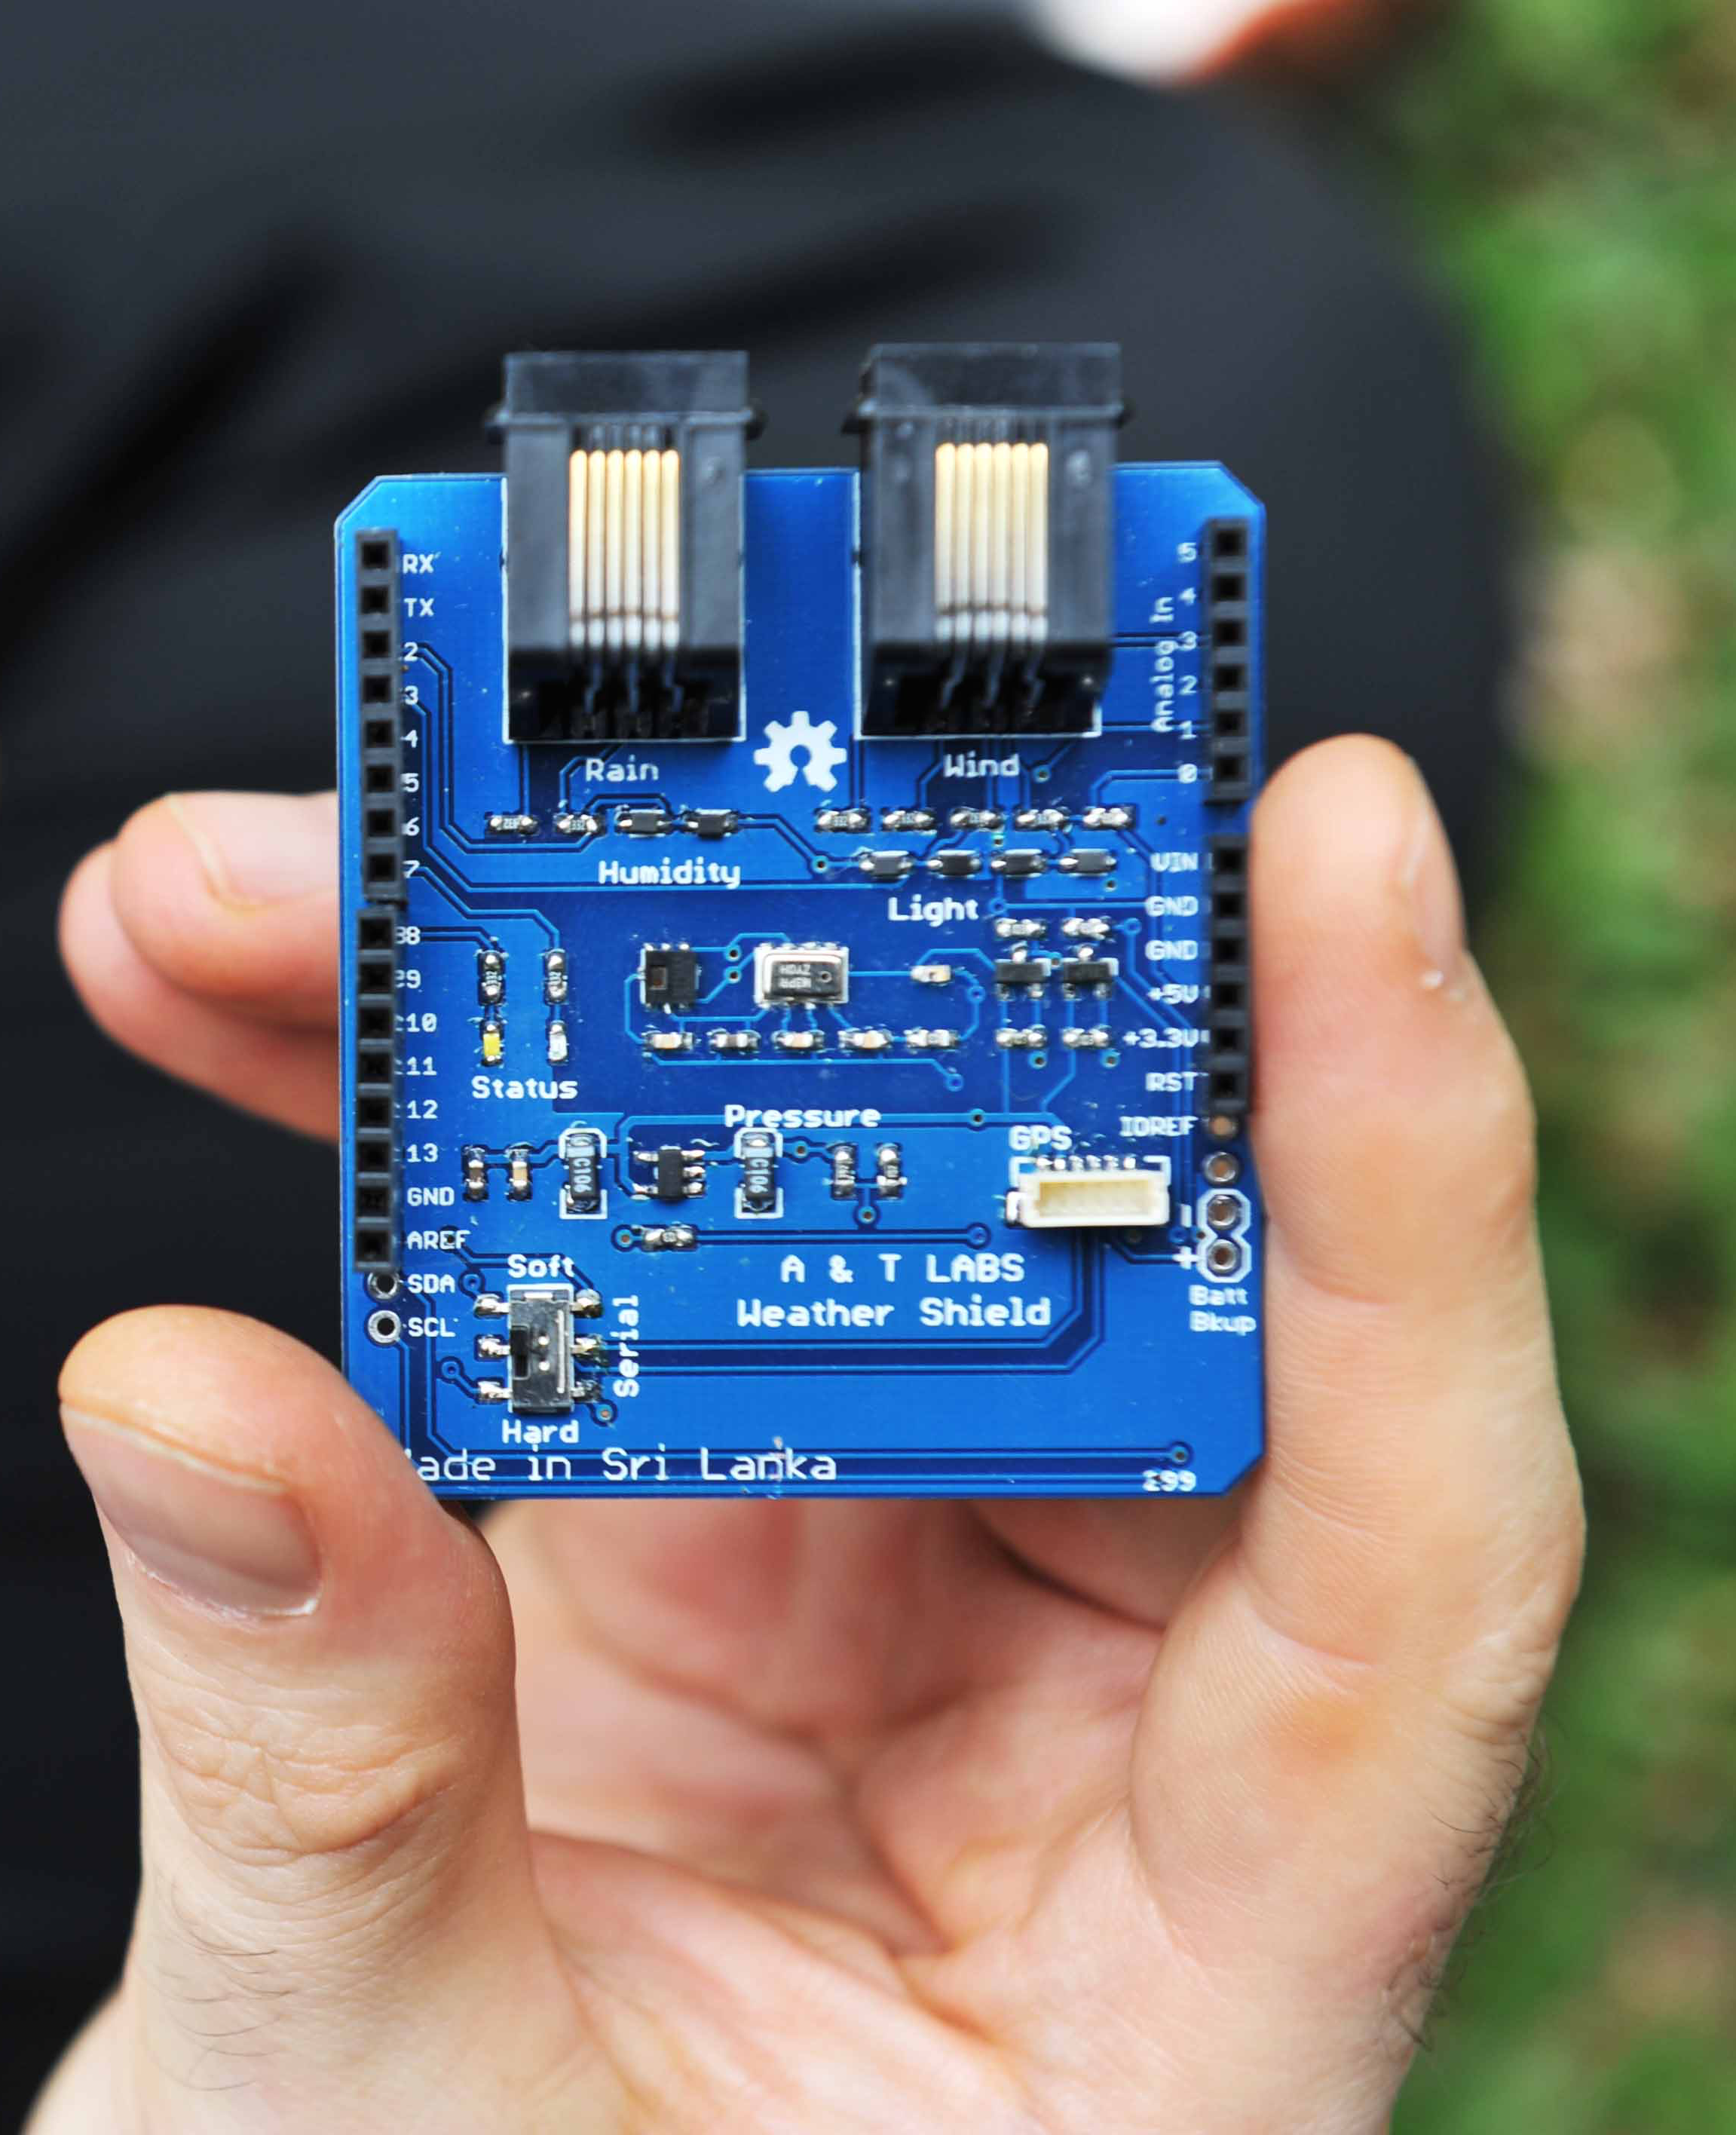
\includegraphics[width=5.5cm]{WeatherShield}\\
\vspace{5mm}
Made in country by a local SME in electronics.\\
Picture credit: Neil Palmer (IWMI)
\end{center}

\end{frame}

\section{Initial work}
\subsection{Irrigation Dept.}
%%%%%%%%%%%%%%%%%%%%%%%%%%%%%%%%%%%%%%%%%%%%%%%%%%%%%%%%%%%%%%%%%%%%
\begin{frame}[fragile]{Set up}

\begin{center}
 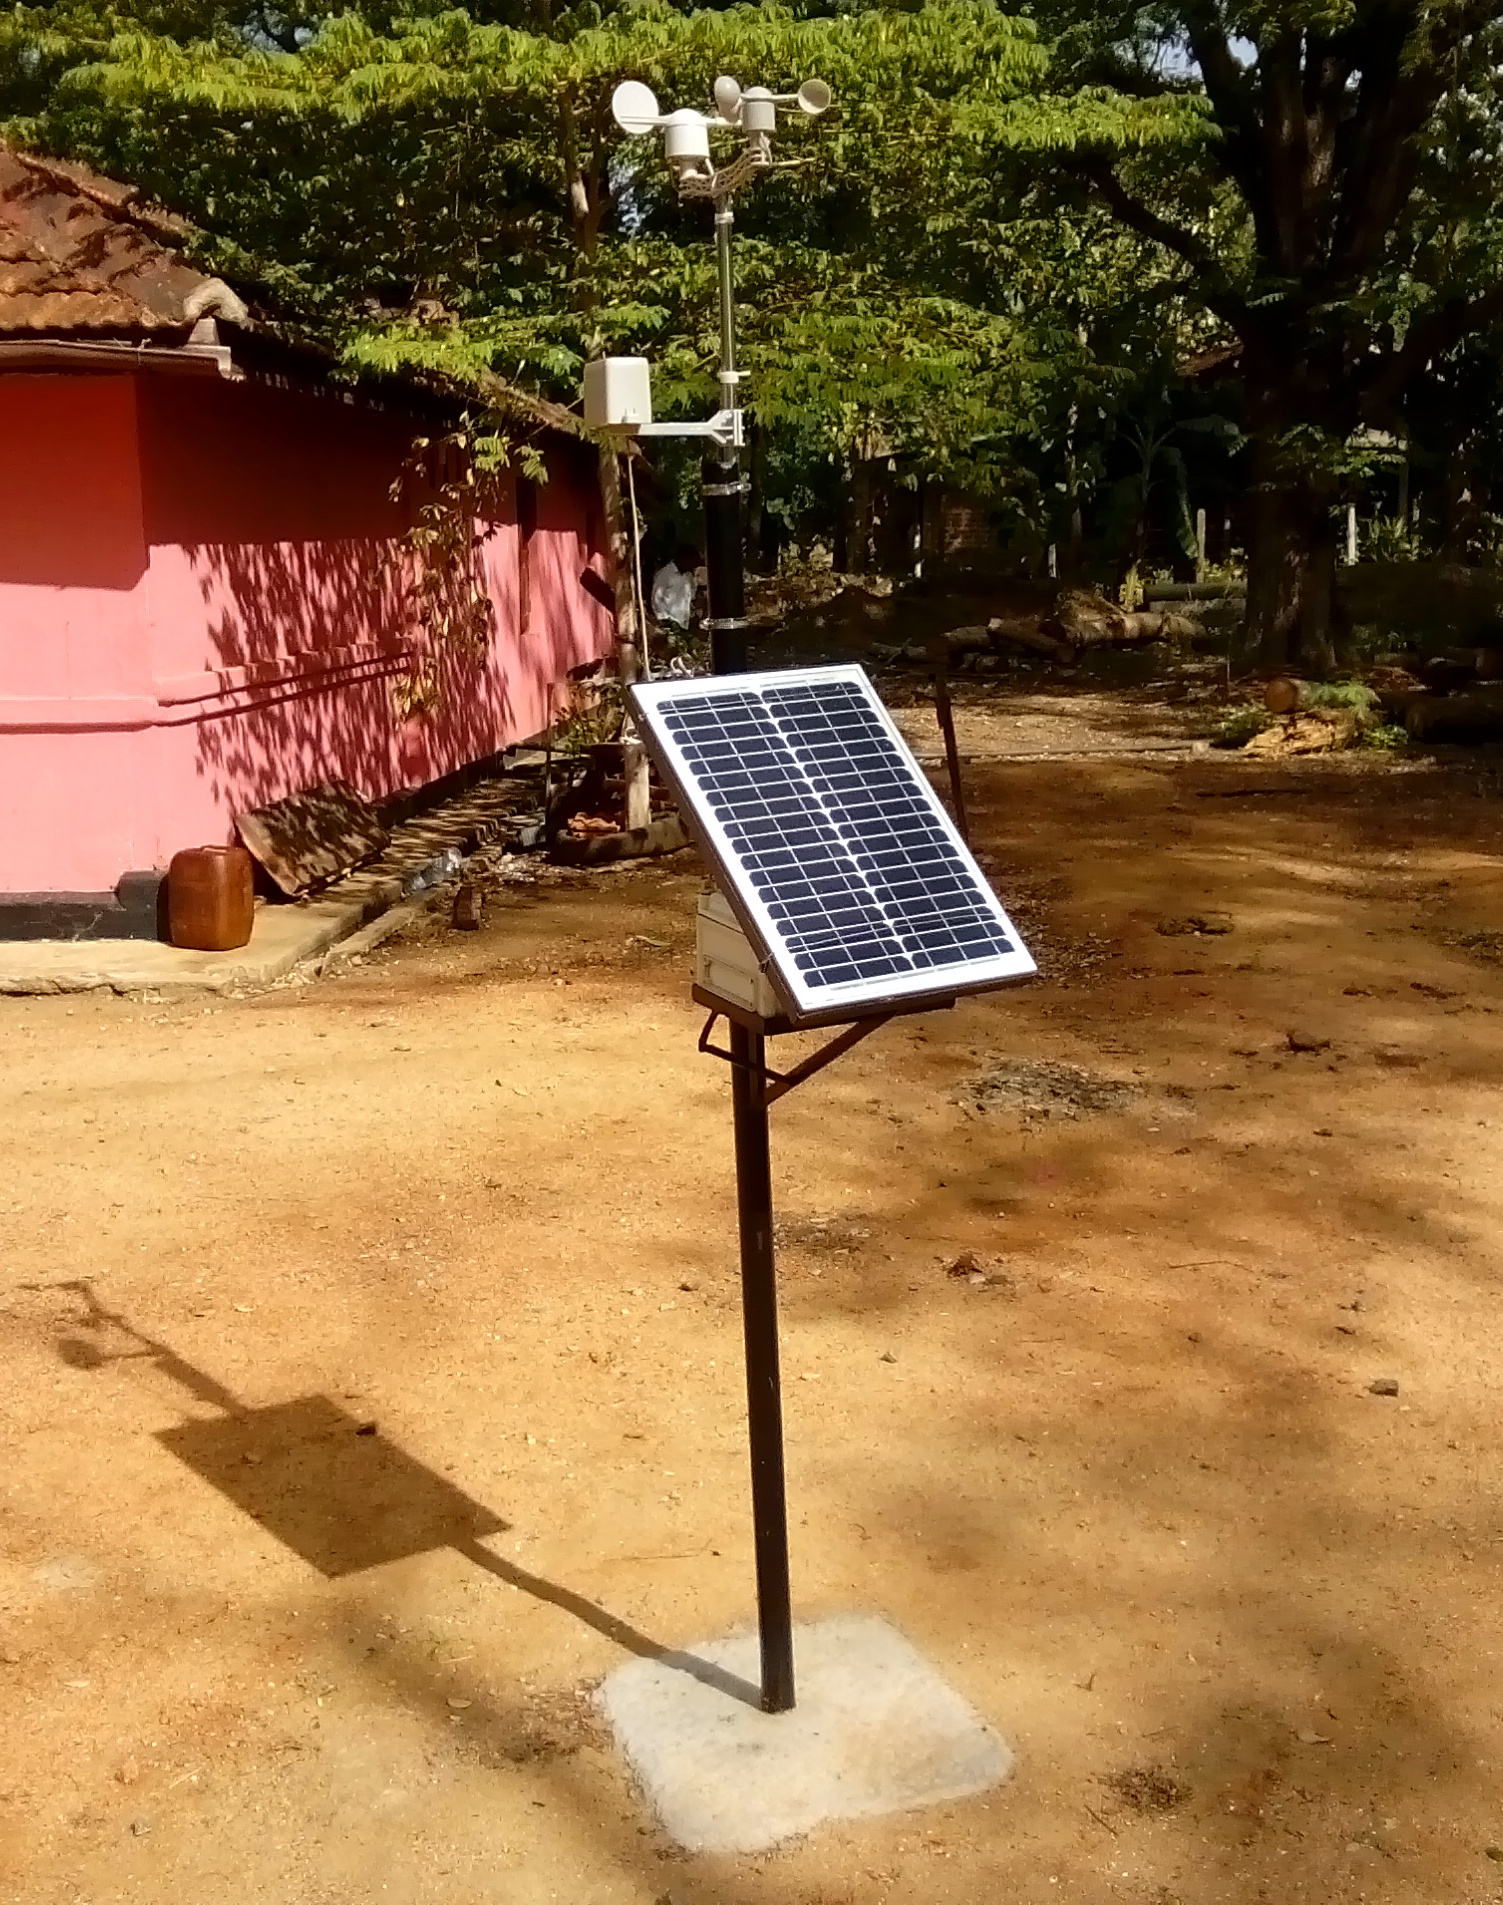
\includegraphics[width=5.5cm]{IMG_20140902_151739}\\
\vspace{5mm}
Picture credit: Niroshan Bandara (UoM)
\end{center}

\end{frame}

\subsection{Met.Dept.}
%%%%%%%%%%%%%%%%%%%%%%%%%%%%%%%%%%%%%%%%%%%%%%%%%%%%%%%%%%%%%%%%%%%%
\begin{frame}[fragile]{Meteorological Department of Sri Lanka}
\begin{center}
 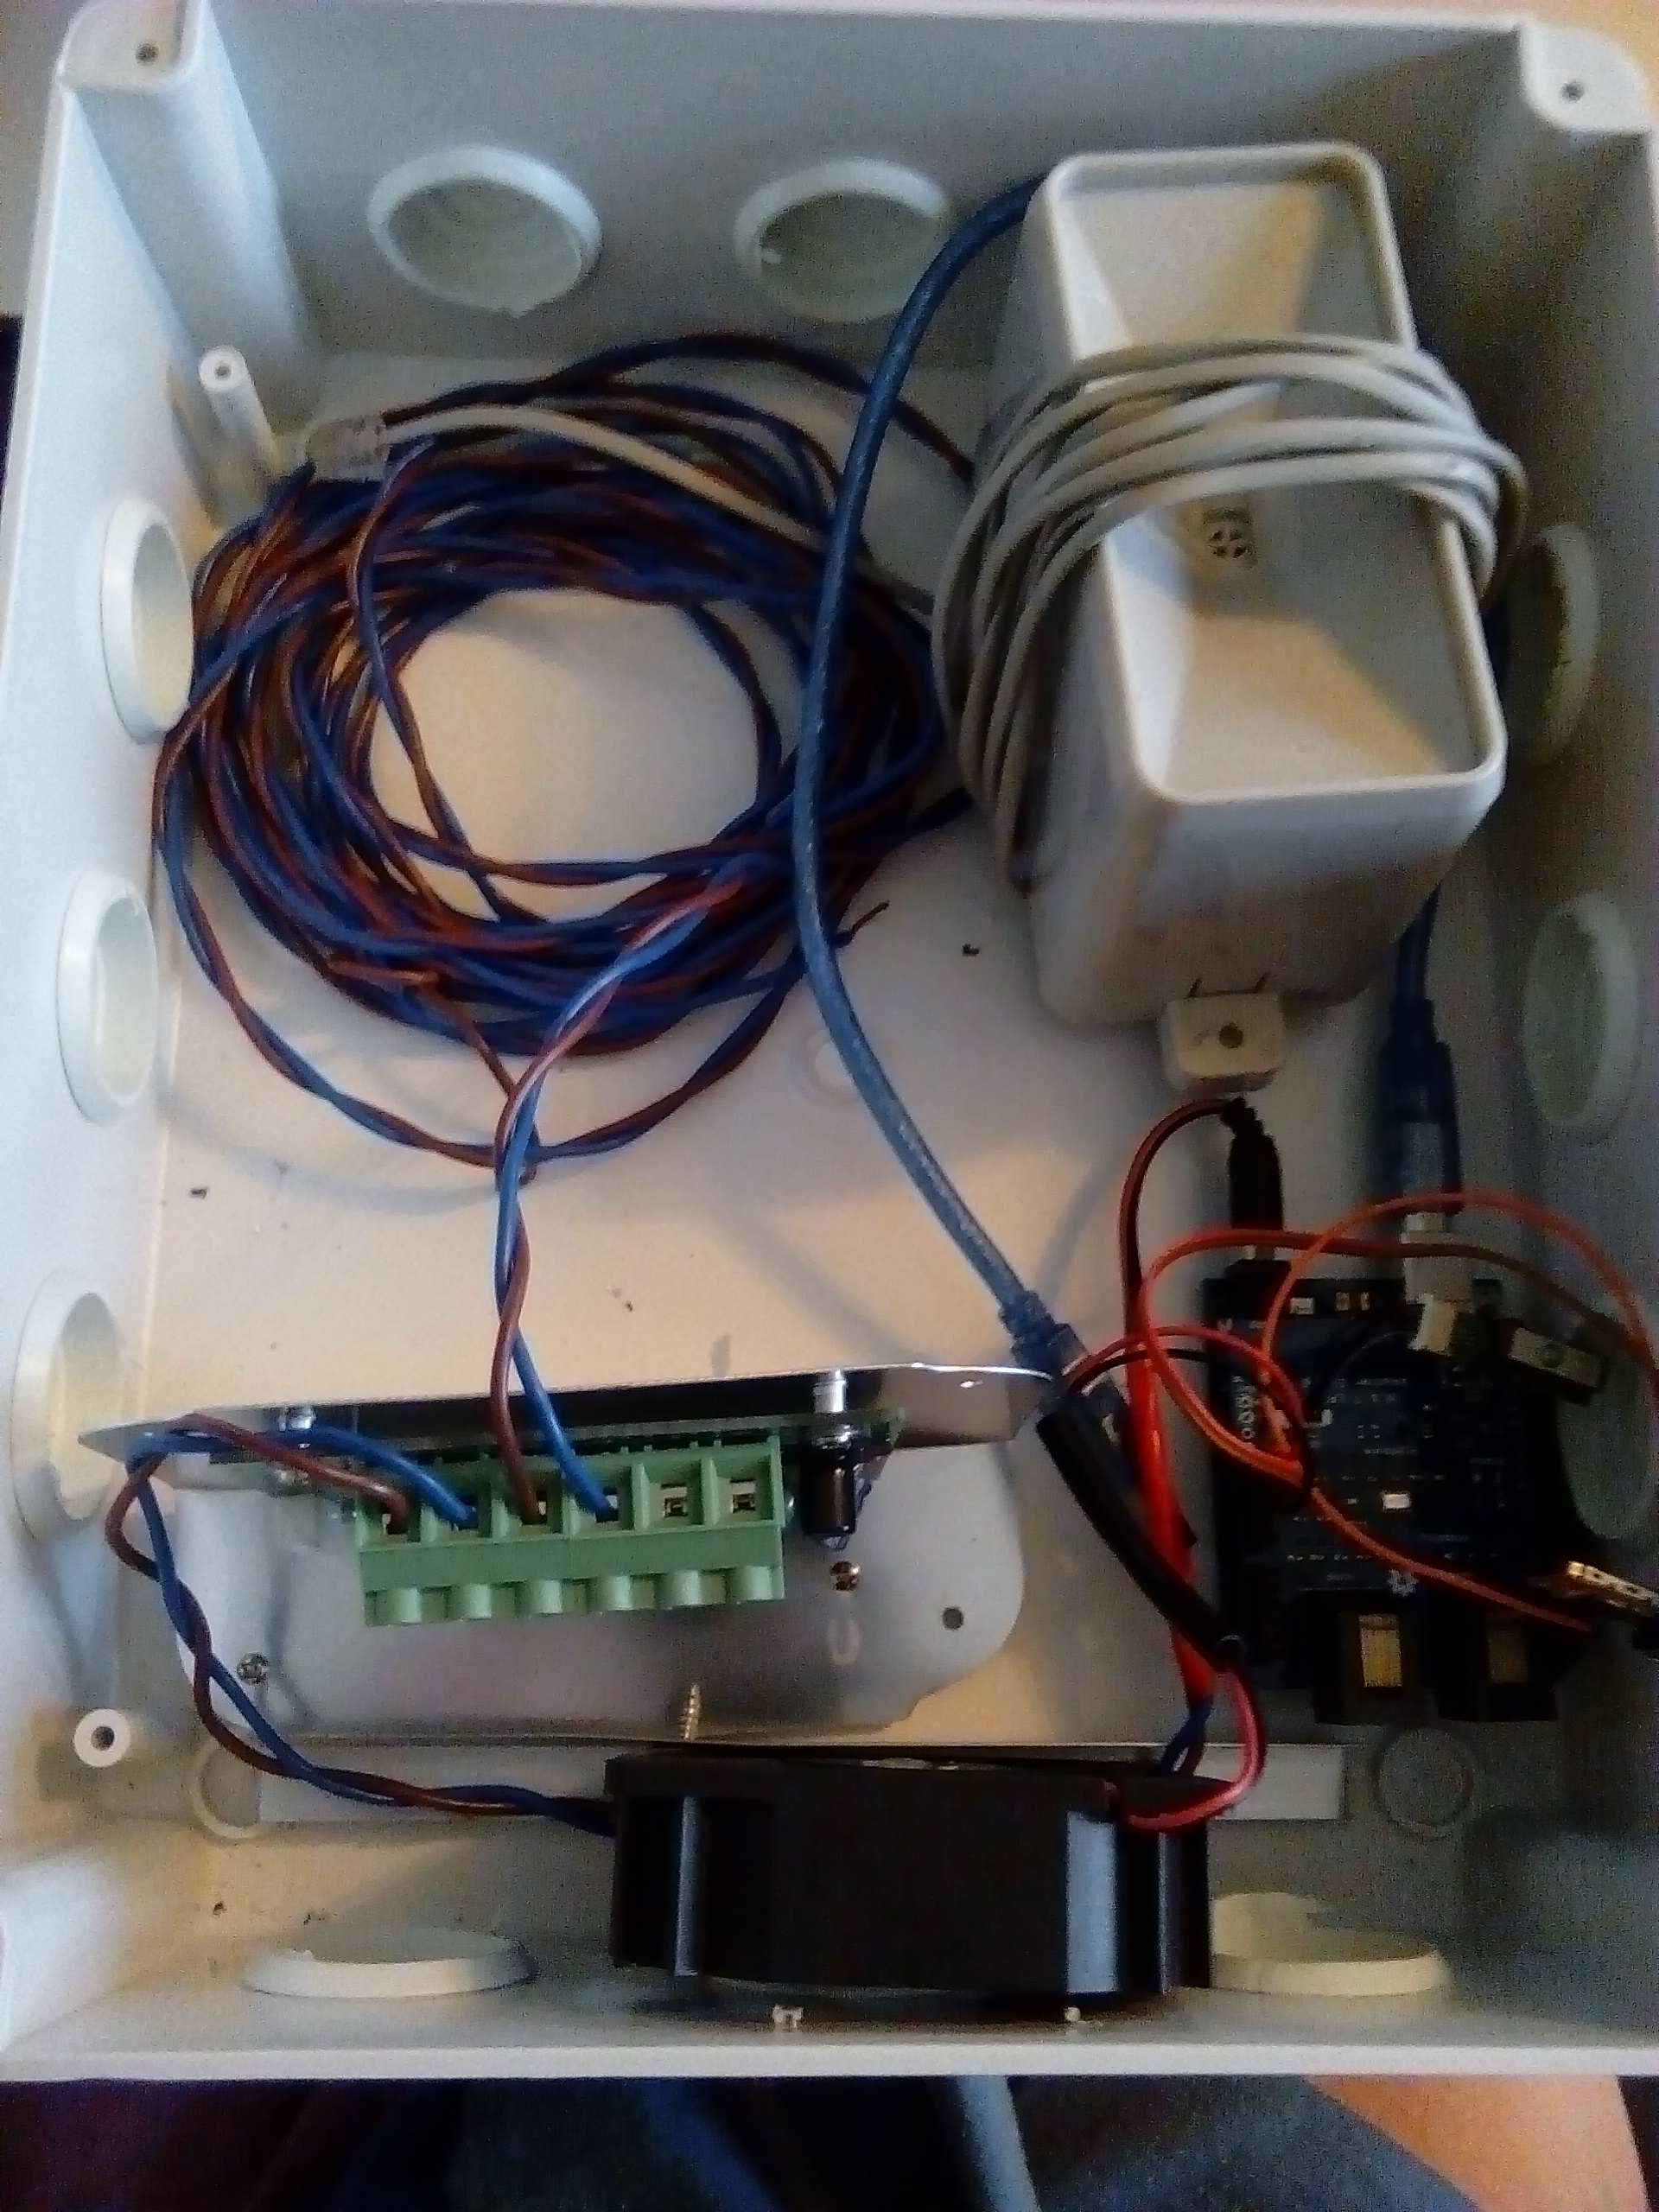
\includegraphics[width=4.5cm]{LKmetdept}
 \hspace{5mm}
 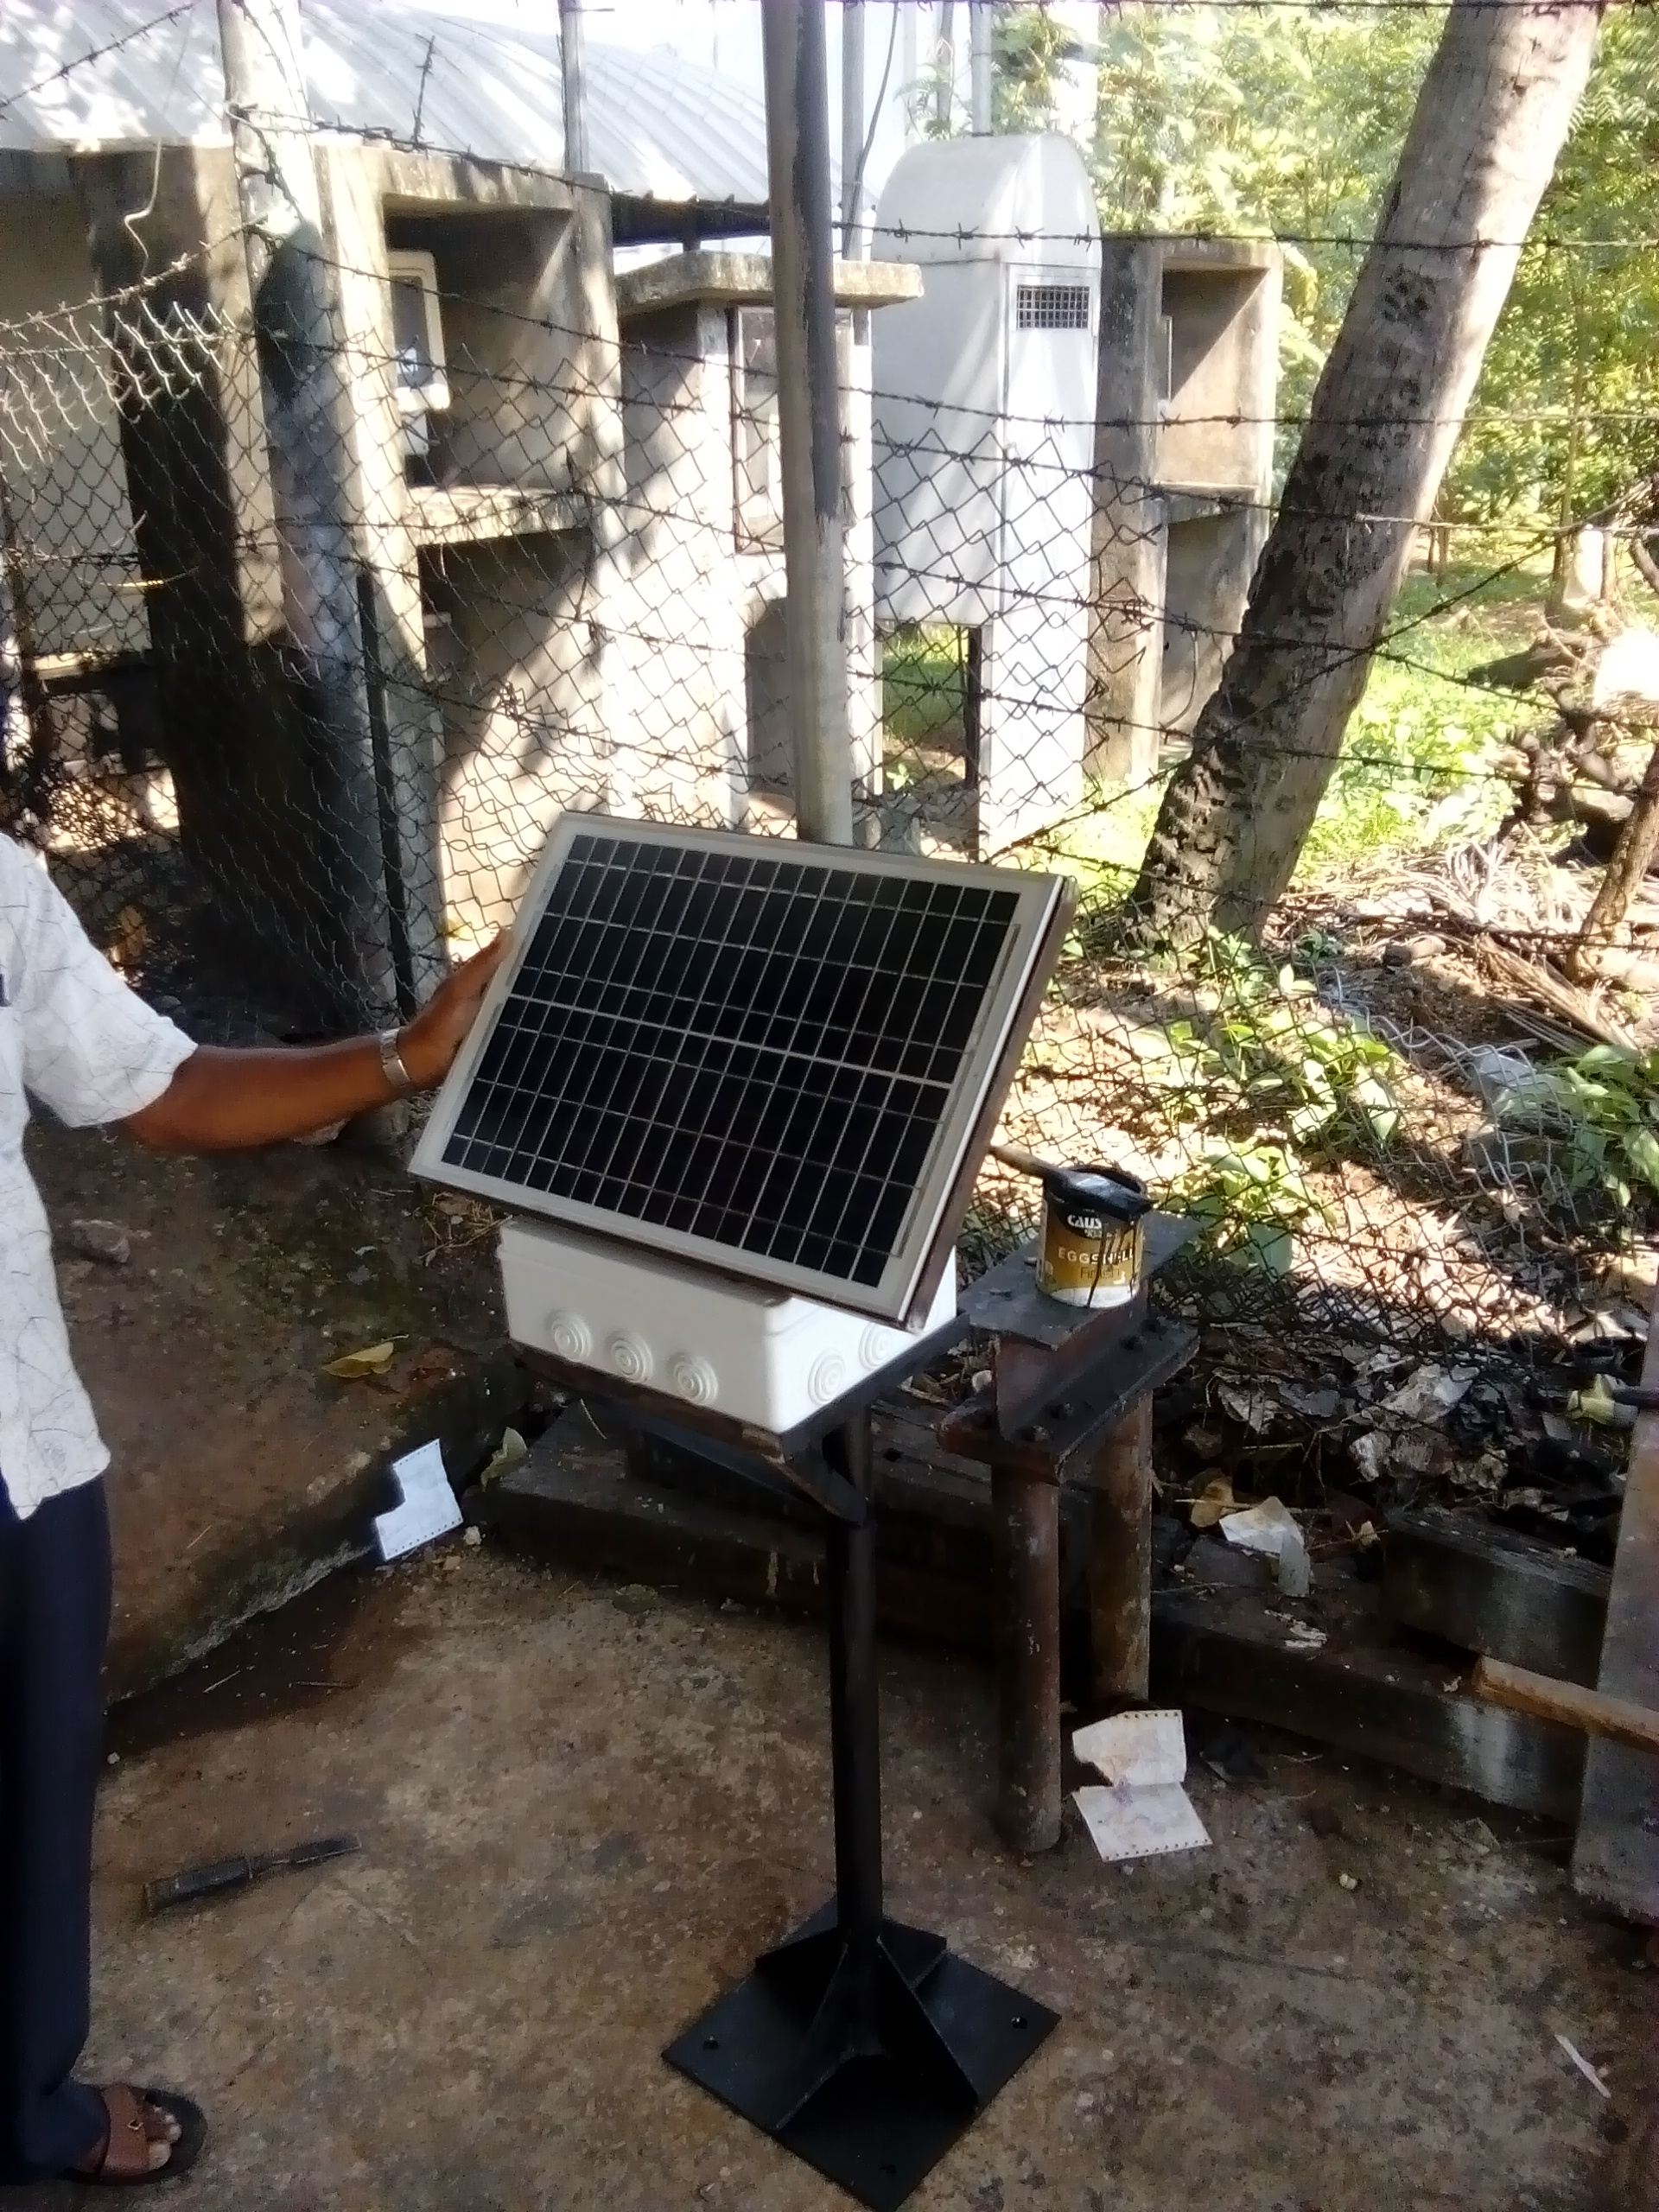
\includegraphics[width=4.5cm]{LKmetdept1}
\end{center}

COSTI (www.costi.gov.lk) is catalizing the proposal for the National Climate Observatory.\\
Test in the Met. Dept. in Colombo (on-going).

\end{frame}

\section{Adoption}
\subsection{LRWHF}
%%%%%%%%%%%%%%%%%%%%%%%%%%%%%%%%%%%%%%%%%%%%%%%%%%%%%%%%%%%%%%%%%%%%
\begin{frame}[fragile]{Lanka Rainwater Harvesting Forum}
\begin{center}
  
\includegraphics[height=2cm]{lrwhf_logo}
 \hspace{2mm}
 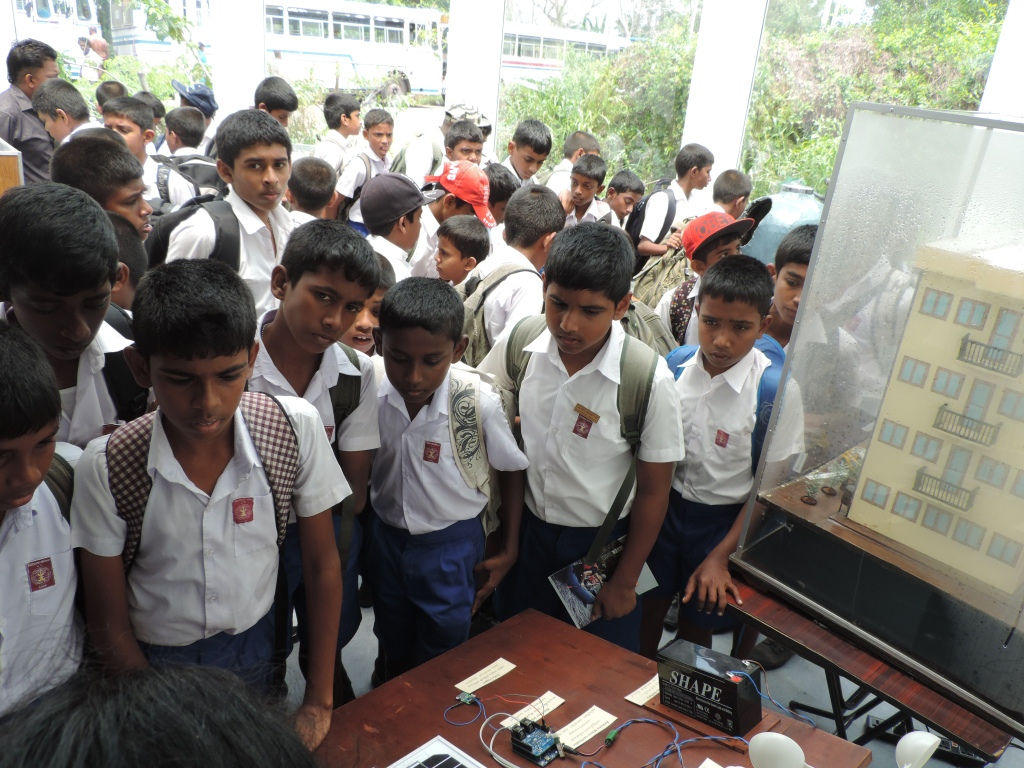
\includegraphics[width=4.5cm]{lrwhf1}
 \hspace{5mm}
 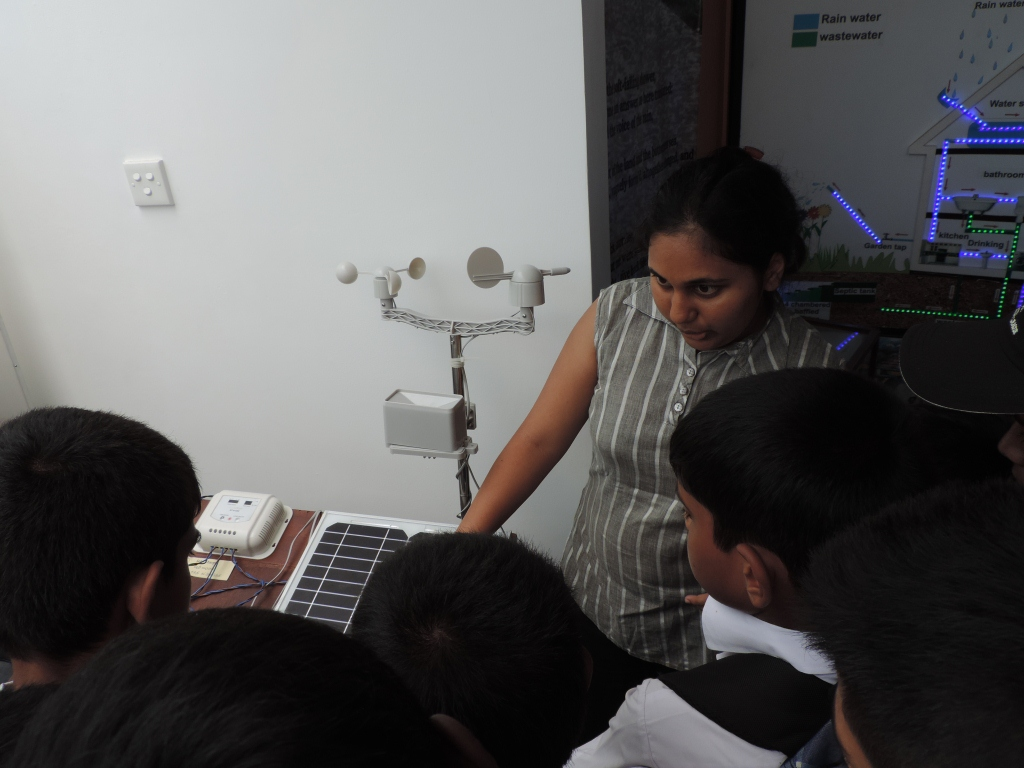
\includegraphics[width=4.5cm]{lrwhf3}\\
\end{center}

LRWHF built 10 units (+5 units for spare parts) under their main USAID project for monitoring the assistance of CKDu stricken villages in drinking rainwater.

\end{frame}

%%%%%%%%%%%%%%%%%%%%%%%%%%%%%%%%%%%%%%%%%%%%%%%%%%%%%%%%%%%%%%%%%%%%
\begin{frame}[fragile]{Lanka Rainwater Harvesting Forum}
\begin{center}
 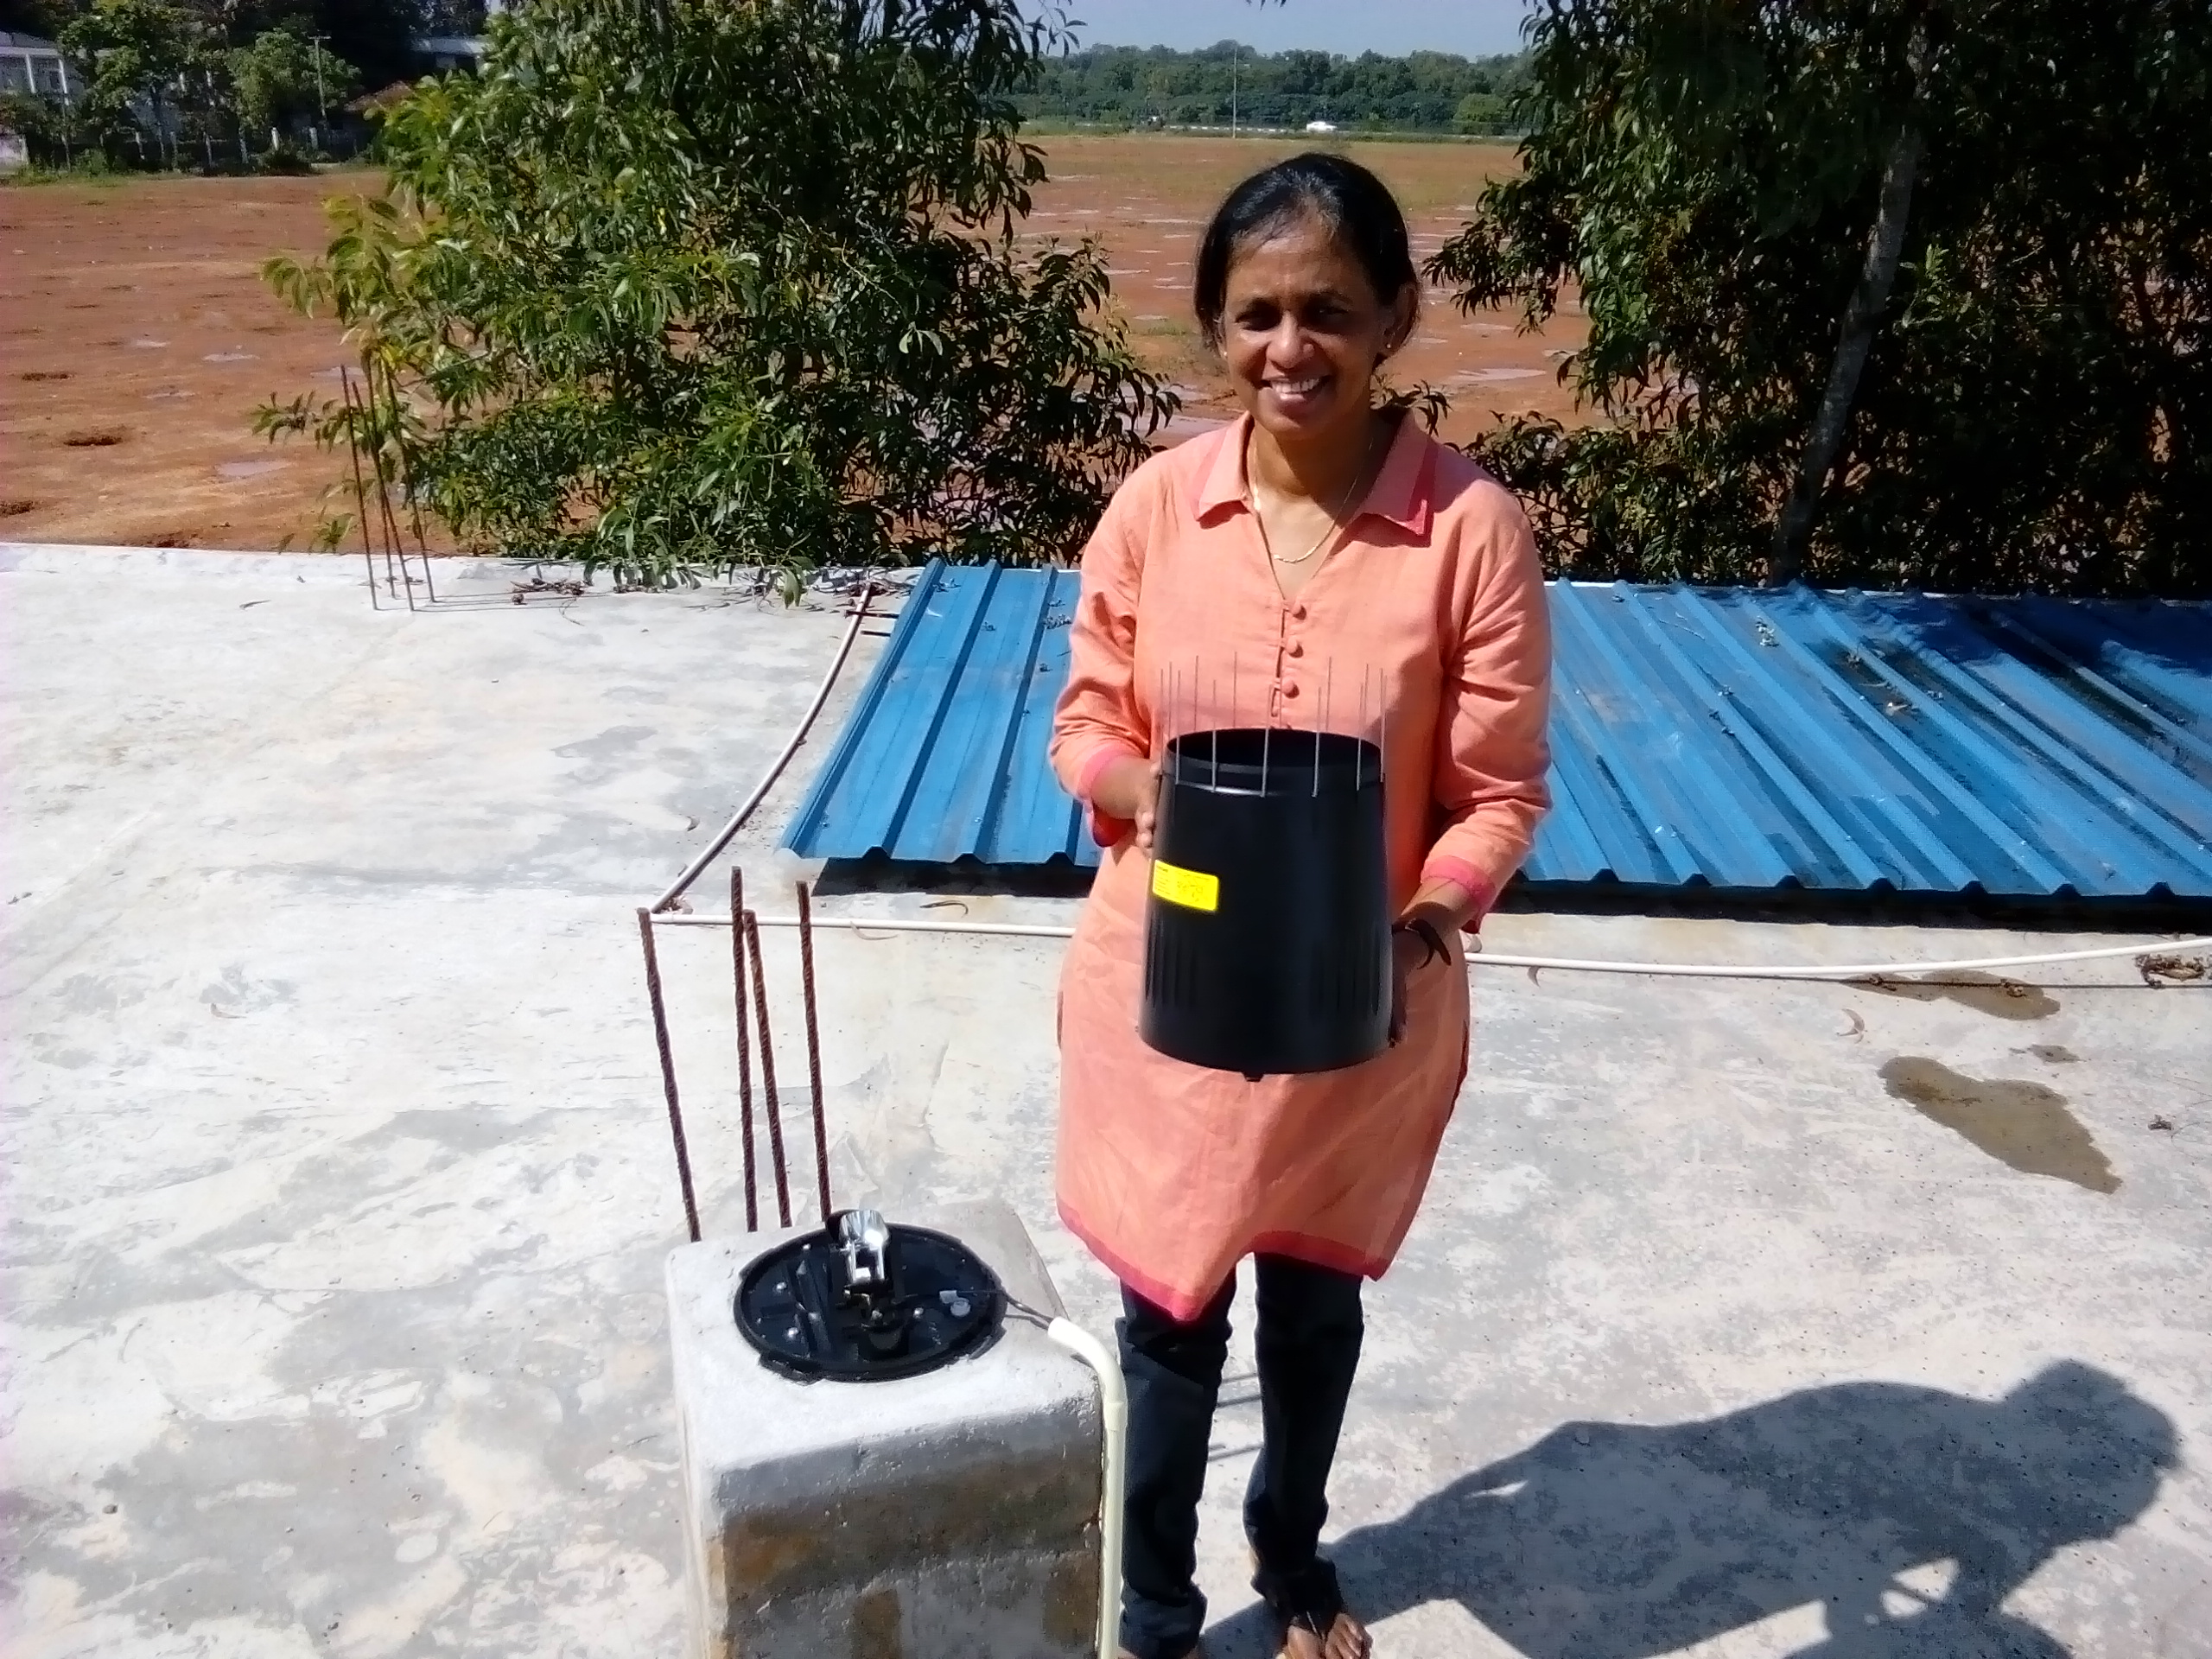
\includegraphics[width=4.5cm]{tanuja1}
  \hspace{5mm}
 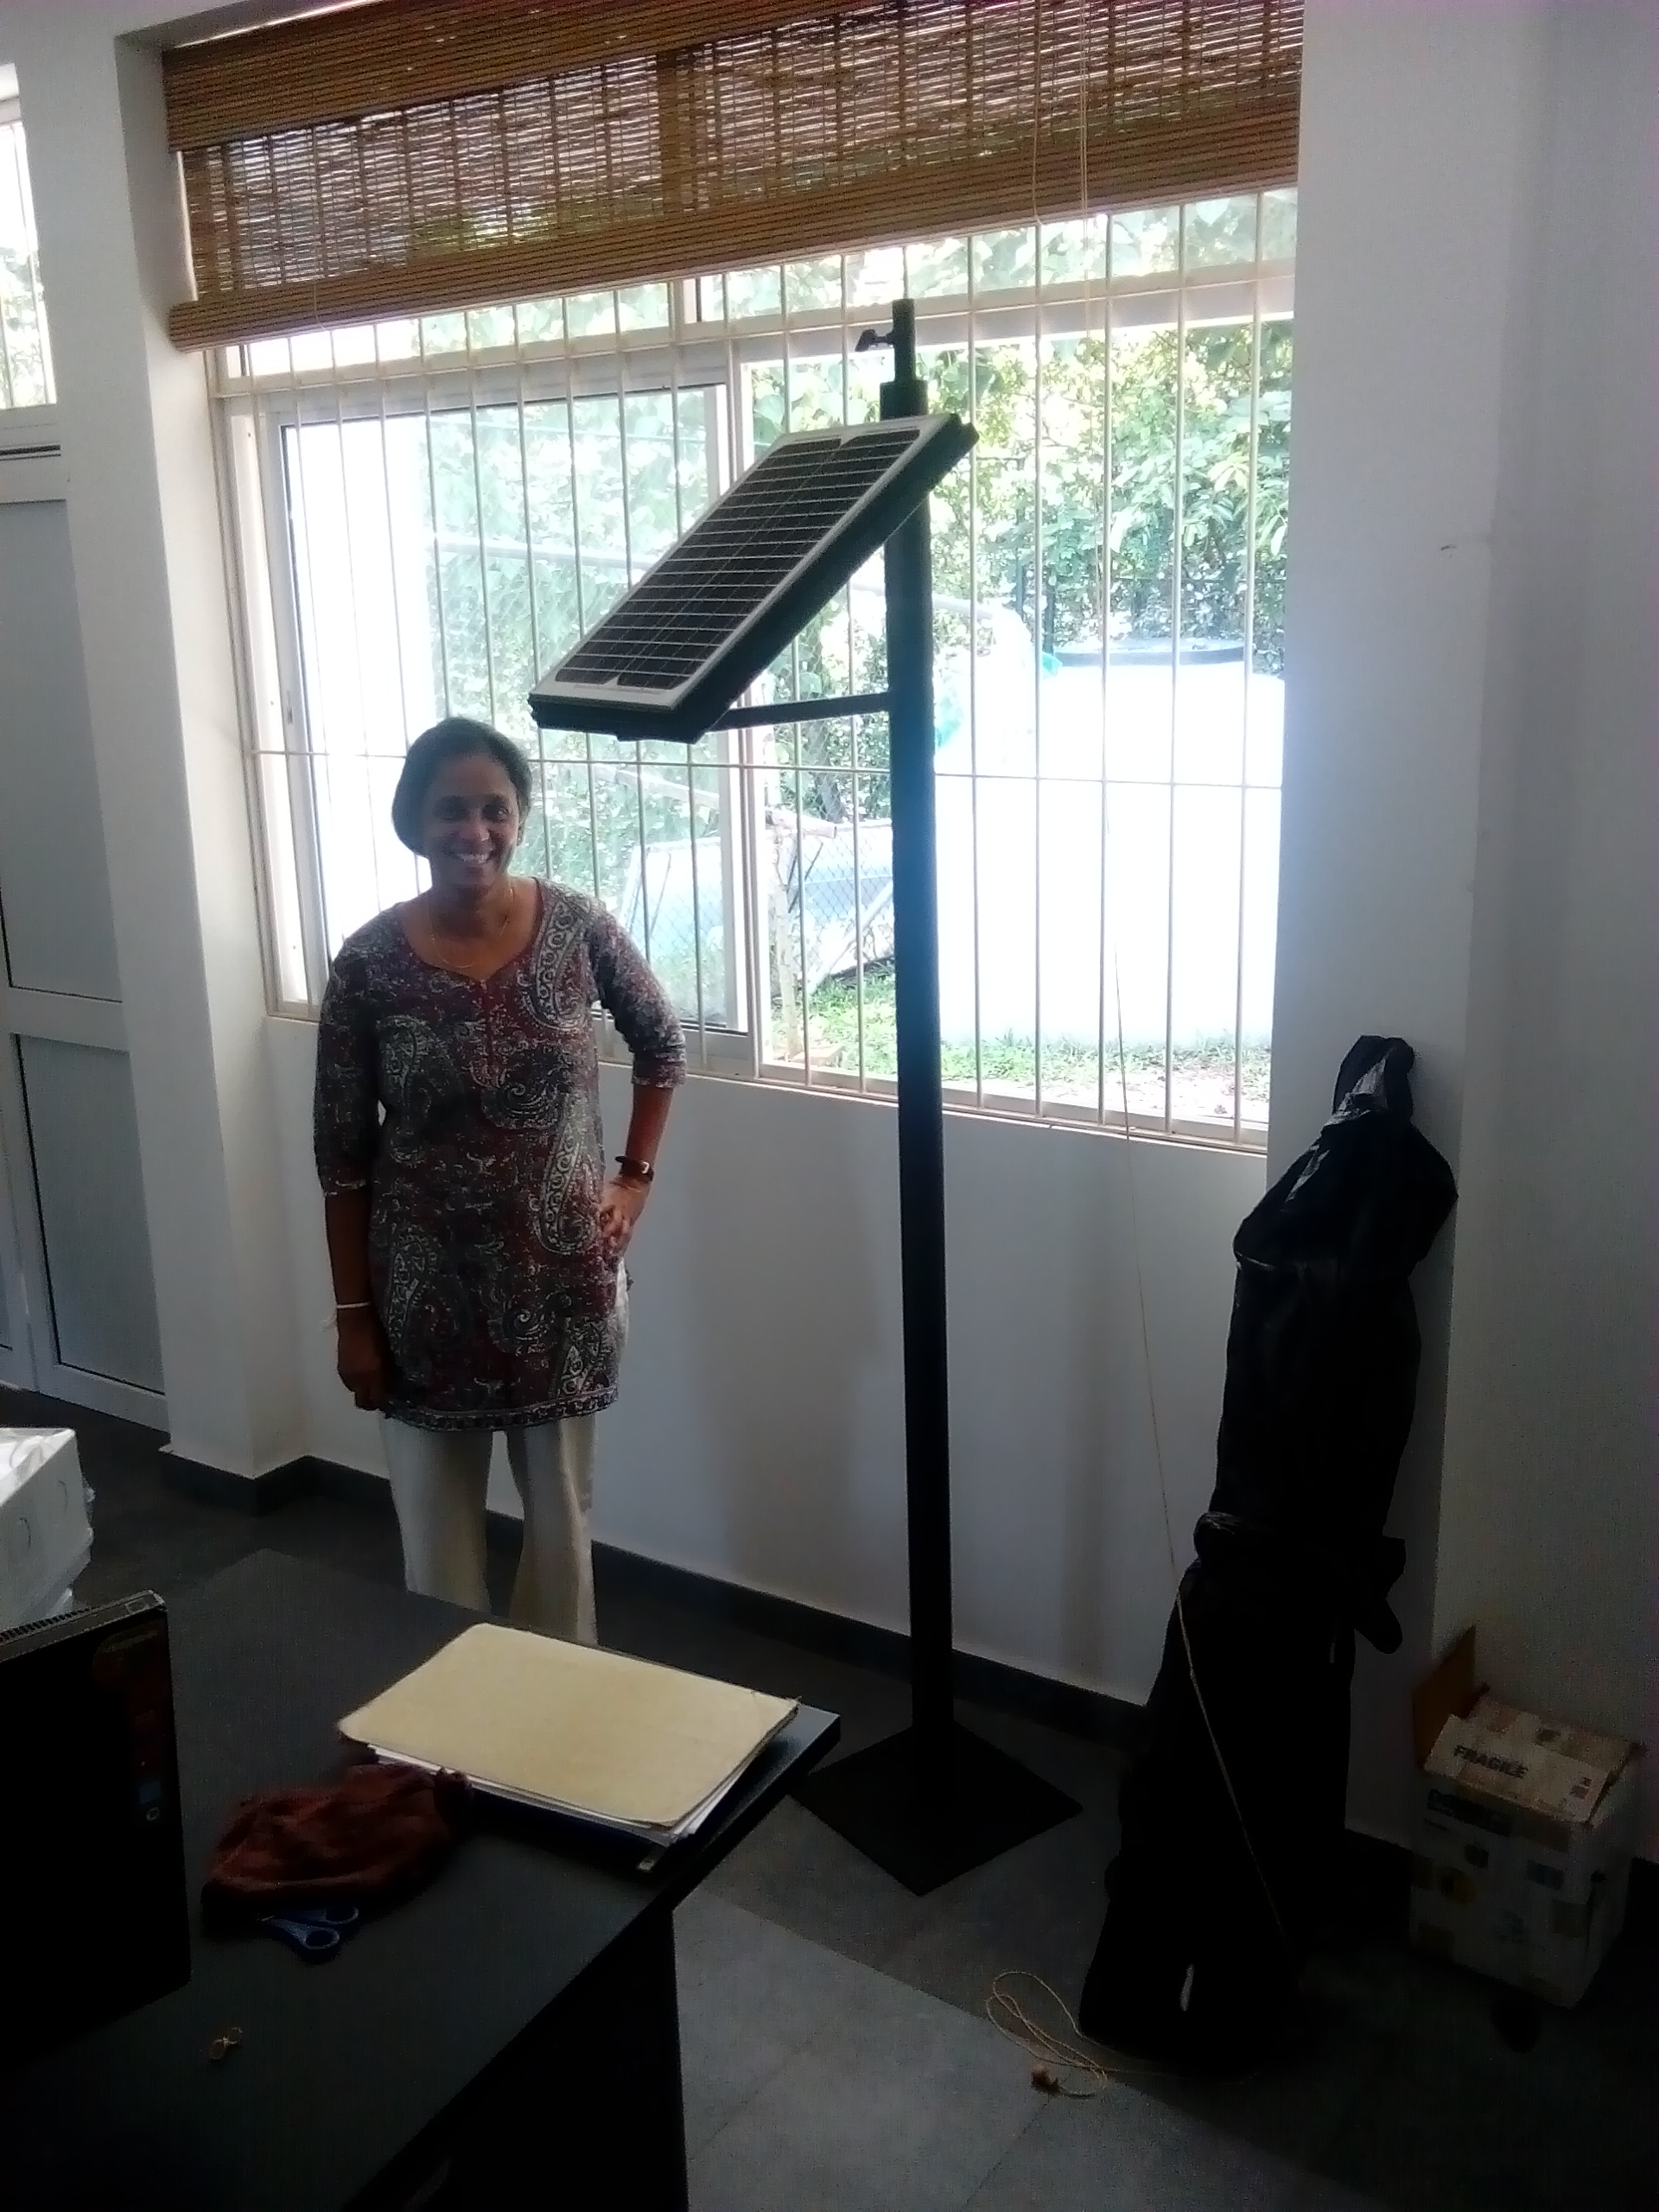
\includegraphics[width=4.5cm]{tanuja2}\\
\end{center}

\begin{center}
Deployment mid-May 2015. \\
Operation/Maintenance trainings, schools \& outreach.
\end{center}

\end{frame}

\subsection{SMEs}
%%%%%%%%%%%%%%%%%%%%%%%%%%%%%%%%%%%%%%%%%%%%%%%%%%%%%%%%%%%%%%%%%%%%
\begin{frame}[fragile]{Electronic SMEs}

Electronic SMEs and start-ups were engaged from the beginning of our search for local availability of components/parts.

\begin{center}
  
\includegraphics[width=8cm]{LK_SMEs}
\end{center}

\end{frame}

\section{Media}
%%%%%%%%%%%%%%%%%%%%%%%%%%%%%%%%%%%%%%%%%%%%%%%%%%%%%%%%%%%%%%%%%%%%
\begin{frame}[fragile]{Media}

 Local and international media helped our business partners marketing outlook and growth.

\begin{center}
  \includegraphics[width=8cm]{MWS_press}
\end{center}

\end{frame}

\section{Future}
%%%%%%%%%%%%%%%%%%%%%%%%%%%%%%%%%%%%%%%%%%%%%%%%%%%%%%%%%%%%%%%%%%%%
\begin{frame}[fragile]{On-going discussions}

\begin{center}
  
\includegraphics[height=3cm]{suparco_logo}
  \hspace{1mm}
  
\includegraphics[height=3cm]{wwf_logo}
  \hspace{1mm}
  
\includegraphics[height=3cm]{undp_logo}  \\
  \vspace{5mm}
  
\includegraphics[height=3cm]{icrc_logo}  \\
  \vspace{3mm}
  
\includegraphics[height=1cm]{wb_logo}
\end{center}

\end{frame}
\section{Conclusions}
%%%%%%%%%%%%%%%%%%%%%%%%%%%%%%%%%%%%%%%%%%%%%%%%%%%%%%%%%%%%%%%%%%%%
\begin{frame}[fragile]{Conclusions}

\begin{block}{An Open Source Hardware/Software\\ Low-Cost Weather Station}
\begin{itemize} 
 \item {\bf Arduino:} Micro-controller 
 \item {\bf Sensors:} Rain, wind, temperature, humidity
 \item {\bf Local:} 80+\% made in the country of use by SMEs
 \item {\bf Local:} Maintenance \& spare parts with local SMEs
 \item {\bf Local:} Local shop sells rural solar power kit
 \item {\bf Local:} Local blacksmith for steel work
\end{itemize}
We work with a rural tank manager from irrigation department for realtime rain alerts.\\Red Cross is evaluating the concept for a project in Togo. Other countries are evaluating for other applications.
\end{block}

\end{frame}

%%%%%%%%%%%%%%%%%%%%%%%%%%%%%%%%%%%%%%%%%%%%%%%%%%%%%%%%%%%%%%%%%%%%
\begin{frame}[fragile]{Thank You}

\begin{center}
 
\includegraphics[height=6cm]{ohm}
\end{center}

\begin{flushright}
 
\includegraphics[height=0.9cm]{iwmi}
 \hspace{5mm}
 
\includegraphics[height=1cm]{uoMoratuwa}
 \hspace{5mm}
 
\includegraphics[height=1cm]{uoMoratuwa_foa}
\end{flushright}

\end{frame}

\end{document}
